\chapter{Thermodynamik}
\label{kap_thermodynamik}


In der Thermodynamik betrachten wir keine kleinste schwingende
Teilchen in der Materie sondern schauen uns die makroskopischen
Eigenschaften -- die \textbf{Zustandsgr"o"sen} (wie Temperatur, Entropie
usw) -- an. 

\paragraph{Absolute Temperatur}
\label{kap_absolute-temperatur}

Wir verwenden eine Temperaturskala, deren absoluter Nullpunkt eine
Naturkonstante ist: Je weiter man ein Gas abk"uhlt, desto geringer ist
sein Dampfdruck. Dabei zeigt sich, dass bei der Temperatur
$\mathbf{-273,15^\circ C}$ \emph{alle Gase den Druck $0$ (Pascal)
haben}.






\section{Zustandsgr"o"sen und Gasgleichung}
\label{kap_zustandsgroessen-und-gasgleichung}


\begin{Def}
   [\index{Zustandsgr"o"sen}Zustandsgr"o"sen] Um einen thermodynamischen
   Gleichgewichts\emph{zustand} eines Systems genau bestimmen zu k"onnen,
   braucht man die vier \emph{Gr"o"sen}
   \begin{itemize}
   \item Temperatur $T$
   \item Volumen $V$
   \item Druck $p$
   \item Entropie $S$
   \end{itemize}
\end{Def}



\paragraph{Ideale Gasgleichung}
\label{kap_ideale-gasgleichung_einfuehrung}

Wir werden uns h"aufig mit der
\index{Ideale-Gas-Gleichung}Idealen-Gas-Gleichung
$$
\boxed { p \cdot V = n \cdot R \cdot T }
$$
besch"aftigen. So ist es wichtig, dass wir die beiden verschiedenen
m"oglichen Formulierungen dieses Satzes in Einklang bringen.

Dazu verwendet man gerne die
\textsc{\index{Avogardro-Konstante}Avogardro} Konstante\footnote{Auch
  manchmal mit $L$ f"ur \textsc{\index{Loschmidt}Loschmidt} abgek"urzt}
$N_A = 6.023 \cdot 10^{ 23 } \frac{1}{\operatorname{mol}}$ und kann so
$R = N_A \cdot K_B$ setzen. So kann man die Gasgleichung
umformulieren:

\begin{equation}
   \label{eq:429}
   \boxed { p \cdot V = N \cdot K_B \cdot T  }
\end{equation}


Dabei ist $p$ der Druck, $V$ das Volumen und $T$ die absolute
Temperatur (s. \ref{kap_absolute-temperatur}) ist. $N$ ist die Anzahl
an Gasteilchen selbst, wobei $n$ die \emph{Anzahl der Mole}
im Gas angibt (Es gilt $N = N_A\, n \approx 6,02\cdot10^{23}
\frac{1}{\operatorname{mol}} \cdot n$.)

Die obere Gleichung wurde \emph{empirisch} gefunden. $R$ wurde hier
als \emph{Proportionalit"atskonstante} eingef"uhrt.







\section{\textsc{Brown}'sche Molekularbewegung und Druck}
\label{kap_brownsche-molekularbewegung}

Gasteilchen fliegen chaotisch durch die Gegend und auch gegen
gr"o"sere Teilchen und die Gef"a"sw"ande.  Sto"sen sie gegen andere,
gr"o"sere, mit dem blo"sen Auge beobachtbare Teilchen und "ubertragen
ihren Impuls auf diese, so nehmen wir das als ungeordnete Bewegung
dieser Teilchen wahr -- das ist die \textbf{\textsc{\index{Brownsche
      Molekulabbewegung}Brown}'sche Molekularbewegung}.

Sto"sen sie dagegen gegen ihre Gef"a"swand, so nehmen wir das als
\emph{Druck} wahr; die mikroskopische Ursache f"ur den Druck ist also
die chatotische Bewegung der Gasteilchen.

Nun kann man untersuchen, wie die Teilchen den (Stempel)Druck ergeben:
Die $N$ Gasteilchen im Volumen $V$ haben die Masse $m$ und bewegen
sich mit der Geschwindigkeit $\vec v = (v_x,v_y,v_z)^T$. Wir
betrachten nur die $x$-Richtung: Hier fliegen die Teilchen mit $v_x$
auf eine Wand der Fl"ache $A$ zu. Dort "ubertragen sie beim Sto"s
(jeweils) den Impuls $\Delta p = 2mv_x$. Es haben $n(v_x)$ Teilchen
die Geschwindigkeit $|v_x|$ (also $\frac{1}{2}n(v_x)$ die
Geschwindigkeit in die gew"unschte Richtung, die andere H"alfte in
Gegenrichtung).

% Auf die Wandfl"ache treffen in einem Zeitintervall $\Delta t$ genau
% $\frac{\frac{1}{2}n(v_x) \cdot v_x}{V}$ Teilchen auf und "ubertragen
% dem Impuls 
% \begin{equation}
% \frac{mv_x^2 \cdot n(v_x)}{V} = \frac{\Delta p}{A \cdot \Delta t}   
% \end{equation}

Im Zeitintervall $\Delta t$ bewegen sich die Teilchen um $\Delta x =
v_x \cdot \Delta t$ weiter. Damit werden alle Teilchen mit der
Geschwindigkeit $v_x$, die sich in dem Volumen $V' = A \cdot v_x \,
\Delta t$ aufhalten, w"ahrend $\Delta t$ gegen $A$ sto"sen. Da die
Teilchen gleich verteilt sind, k"onnen wir annehmen, dass der Quotient
$\frac{V'}{V}$ von diesem Volumen zum Gesamtvolumen dem Quotienten von
Teilchen mit $v_x$ innerhalb von $V'$ zu Teilchen mit $v_x$ insgesamt
im Volumen $V$ entspricht:
\begin{equation*}
  \frac{V'}{V} =  \frac{A \cdot v_x \, \Delta t}{V} = \frac{n(v_x,
    \text{in }V')}{n(v_x)} = \frac{n'(v_x)}{n(v_x)}
\end{equation*}
Von diesen $n'(v_x)$ Teilchen bewegt sich nun die H"alfte in die
"`richtige"' Richtung und damit wird (wenn jedes Teilchen $\Delta p =
mv_x$ "ubertr"agt) insgesamt von den Teilchen mit $v_x$ der Impuls
\begin{equation}
     \label{eqn_Impuls_eines_teilchens}
   \Delta  p^\Sigma = \Delta p \cdot \frac{1}{2}n'(v_x) = 
\frac{1}{2} \cdot 2m v_x \cdot \frac{A \cdot v_x \cdot \Delta t}{V}
\cdot n(v_x)
\end{equation}
"ubertragen. Dies Teilt man nun noch durch $\Delta t$ und $A$ und
erh"alt
\begin{equation}
   \label{eq:206}
   \frac{\Delta p^\Sigma}{A \cdot \Delta t} = \frac{mv_x^2 \cdot n(v_x)}{V}
\end{equation}
%
F"ur kleine $\Delta t$ gilt nun $\Delta t \to \diff t$ und $\Delta p^\Sigma
\to \diff p^\Sigma$. Also f"ur den Impuls aus Gl. \eqref{eqn_Impuls_eines_teilchens}:
$$
\frac{\diff p^\Sigma}{A \cdot \diff t} = 
\frac{\diff }{\diff t } p^\Sigma \cdot \frac{1}{A}
%
%\frac{\diff (mv)}{\diff t A} = \frac{m\ddot x}{A} 
= \frac{F}{A} = P
$$
wobei $P$ der (messbare) Gesamtdruck ist.\footnote{Normalerweise
  bekommt der Druck das Formelzeichen $p$ -- in diesem Falle wurde $P$
gew"ahlt, damit man ihn vom \emph{Impuls} $p$ unterscheiden kann.} D.h. dieser
Druck $P$
resultiert einzig aus den Gasteilchen, die mit $v_x$ gegen die eine
Wand sto"sen.

Betrachtet man nun alle Geschwindigkeiten, so gilt mit
Gl. \eqref{eq:206}:
\begin{equation}
   \label{eqn_allge_geschwindigkeiten}
   P = \int_{ v_x = -\infty }^{ v_x = + \infty } \frac{mv_x^2 \cdot
     n(v_x)}{V} \diff v_x = 
\frac{m \bar v_x^2 \cdot N}{V}
\end{equation}
Dabei ist $\bar v_x$ die \emph{Durchschnittsgeschwindigkeit}:
$$
\bar v_x^2 = \int_{ v_x = - \infty }^{ v_x = + \infty } v_x^2 \cdot
{\frac{n(v_x)}{N}} \diff v_x
$$
Der Quotient $\frac{n(v_x)}{N}$ kann als Wahrscheinlichkeit, dass ein
Teilchen die Geschw. $v_x$ hat, interpretiert werden. (Oder man sagt,
dass die Summe "uber alle Teilchen, gewichtet mit dem
Geschwindigkeitsquadrat, gebildet ($\bar v^\Sigma = \sum_{i = 1}^N
(v_x^{(i)})^2$) wird und
anschlie"send das mittlere Geschwindigkeitsquadrat, indem man durch die
Anzahl an Teilchen teilt ($\bar v = \frac{\bar v^\Sigma}{N}$).)

Nehmen wir eine isotrope Teilchenbewegung an (also dass keine Richtung
ausgezeichnet ist), so folgt $\bar v_x^2 = \bar v_y^2 = \bar v_z^2$ und
mit
$
\bar v^2 := \bar v_x^2 + \bar v_y^2 + \bar v_z^2
$
folgt
$$
\bar v_x^2 = \frac{\bar v^2}{3}
$$
Setzt man dies in Gl \eqref{eqn_allge_geschwindigkeiten} ein, so
ergibt sich
\begin{equation}
   \label{eqn_Druck}
   P = \frac{m \bar v^2 N}{3 V} =
\boxed{ \frac{2}{3} \frac{N}{V} \cdot \underbrace{\frac{m \bar
      v^2}{2}}_{\bar u} = P }
\end{equation}
Dabei ist  ${\bar u}$ die \textbf{Mittlere kinetische Energie
  eines Teilchens}\index{Mittlere kinetische Energie}.

Nun betrachten wir $N = L$ Teilchen (mit $\mathbf{ L = 6,023 \cdot
  10^{ 23 } = 1 \operatorname{mol}}$) setzen unsere Formel f"ur Druck
(Gl. \eqref{eqn_Druck}) in die \emph{ideale Gasgleichung} ein, so
erhalten wir
\begin{equation}
   \label{eqn_bolzmann-herleitung}
   PV = RT \mathbf = 
\frac{2}{3} L \bar u ~ ~ \Rightarrow ~ ~ 
\bar u = \frac{3}{2} \left( \frac{R}{L} \right ) T = \boxed{\frac{3}{2}
 {K_B} T = \bar u}
\end{equation}
Wir haben hier die
\textbf{\textsc{\index{Boltzmann}Boltzmann}-Konstante}
definiert:

\begin{Def}[\textsc{Boltzmann}-Konstante $K_B$]
$$
\frac{R}{N_A} = {K_B} = 1,38 \cdot 10^{ -23 } \,
\frac{\operatorname{J}}{\operatorname{K}}
$$
\end{Def}
(Die \index{universelle Gaskonstante}universelle (oder \index{molare
  Gaskonstante}molare) Gaskonstante $R$ hat die Einheit $[R] =
\frac{\operatorname{J}}{\operatorname{mol}\cdot \operatorname{K}}$ und
$R = 8.31 \frac{\operatorname{J}}{\operatorname{mol}\cdot \operatorname{K}}$.)

Au"serdem haben wir dadurch, dass $\bar u$ die mittlere kinetische
\emph{Energie} eines Teilchens ist, in Gl
\eqref{eqn_bolzmann-herleitung} gesehen, dass auf der rechten Seite
der Gleichung auch eine \emph{Energie} stehen muss:
\begin{Def}[\index{Thermische Energie}\index{Innere Energie}Innere Energie $U$]
   Die Innere Energie (auch "`Thermische Energie"') eines K"orpers
 ist
   \begin{equation}
      \label{eqn_thermische-energie}
      \boxed{ U = \frac{f}{2} \cdot N \cdot K_B \cdot T }
   \end{equation}
   weil die Thermische Energie eines Teilchens $u = \frac{f}{2} \cdot
   K_B \cdot T$ ist und der K"orper $N$ Teilchen hat.
\end{Def}




\paragraph{Beachtung der Freiheitsgrade}
\label{kap_beachtung-freiheitsgrade}

Dabei haben wir in unserer Rechnung noch eine Vereinfachung gemacht;
der Faktor $\frac{3}{2}$ in Gl \eqref{eqn_bolzmann-herleitung} kommt
daher, dass wir als Teilchenbewegungen nur \emph{Translationen} (also
gewisserma"sen Verschiebungen) in den drei Raumrichtungen zugelassen
haben. Die Teilchen k"onnen aber auch noch "uber andere Energieformen
verf"ugen. 

Dies "au"sert sich mathematisch in der 
\begin{Def}[Zahl der \index{Freiheitsgrade}Freiheitsgrade]
   Die Zahl $f$ gibt an, wie viele Bewegungsarten mit Energie
   verkn"upft sind. M"oglich ist dabei u.a.
   \begin{itemize}
   \item Translation 
\item Rotation
\item Schwingungen
   \end{itemize}
\end{Def}
Dabei kann ein \textbf{punktf"ormiges Molek"ul} wirklich nur drei Freiheitsgrade
haben, weil f"ur eine Rotation keine Energie ben"otigt wird, ebensowenig
kann das Teilchen schwingen: ${f = 3}$, wie in unserer Formel
\eqref{eqn_bolzmann-herleitung}.

Betrachtet man aber \textbf{mehratomige Molek"ule} -- bspw. Sauerstoff $O_2$ --,
so kann hier neben den drei Translationen noch \emph{Rotationen} um
zwei Achsen stattfinden (die Translation um die L"angsachse ist wieder
nicht mit Energie verbunden) und au"serdem noch eine \emph{Schwingung}
-- eben l"angs der L"angsachse. F"ur die Z"ahlung der Freiheitsgrade
m"ussen wir diese aber \emph{doppelt} z"ahlen, weil neben der
Schwingungsenergie auch noch \emph{potentielle} Energie durch die
Anziehungskr"afte der Teilchen gegeneinander auftritt, die vom Betrag
her so gro"s ist, wie die Bewegungsenergie beim Schwingen. Der
Freiheitsgrad eines solchen Teilchens w"are also ${f =
  7}$. In Rechnungen vernachl"assigt man die Schwingung aber gerne,
weil sie bei Raumtemperatur sehr klein ist: ${f = 5}$.

Zus"atzlich "andern sich die Freiheitsgrade je nach
\textbf{Anregungszustand} der Teilchen; bei tiefen Temperaturen
bspw. rotieren die Teilchen kaum und so ist $f = 3$. Steigt die
Temperatur, rotieren sie st"arker, und so erh"alt man bspw. $f =
5$. Bei noch weiterer Erw"armung kommt dazu noch die Schwingung, die
zweitere Freiheitsgrade aufaddiert -- also bspw auf $f = 7$.

Die Zahl der Freiheitsgrade muss keine ganze Zahl sein: Wie oben
beschrieben h"angt sie stark von Temperatur ab. Da die Temperatur eine
\emph{kontinuierliche} Gr"o"se ist (also "`flie"sen"' von einer zur
n"achsten Gr"o"se geht) sollte die Zahl der Freiheitsgrade dies auch tun
-- und dazu \emph{muss} $f \in \mathbb R$ liegen. 


\paragraph{Zusammenhang kinetische Energie -- Thermische Energie}
\label{kap_zusammenhang-kinetische-energie-thermische}

Wir finden "uber diese Freiheitsgrade den Zusammenhang, den wir in
Gl. \eqref{eqn_bolzmann-herleitung} schon f"ur ideale Gase mit $f = 3$
gesehen haben:
\begin{equation}
   \label{eqn_kinetische-energie}
   \boxed{ \bar u = \frac{f}{2} \cdot K_B \cdot T }
\end{equation}
Die Energie des Gasteilchens liegt vollst"andig als kinetische Energie
vor.\footnote{Es kann ja keine Spannenergie haben, die Potentielle Energie wird
in diesem Kapitel nicht betrachtet.} Damit ist $\bar u$ gleichzeitig
die Kinetische Energie, und f"ur ein Teilchen gilt:
\begin{equation}
   \label{eq:434}
   \frac{1}{2} m \bar v^2 = \bar u \text{ und damit } ~ \bar v =
   \sqrt{\frac{f K_B T}{m}}
\end{equation}
Dabei ist $\bar v$ die mittlere Geschwindigkeit eines Teilchens.





\section{Thermische Eigenschaften von Materie}
\label{kap_thermische-eigenschaften-von-materie}

\begin{Def}[\index{Spezifische W"armekapazit"at}\index{Spezifische W"arme}Spezifische W"arme(kapazit"at)]
   Um die Temperatur eines K"orpers um $\Delta T$ zu "andern, braucht
   man die W"arme $\Delta Q$ mit
   \begin{equation}
      \label{eqn_spez-waerme}
      \boxed{\Delta Q = c \cdot m \cdot \Delta T}
   \end{equation}
   dabei ist $c$ die \textbf{Spezifische W"arme}(kapazit"at) und eine
   Eigenschaft des K"orpers.
\end{Def}

M"ochte man eine Gr"o"se verwenden, die von der Teilchenzahl unabh"angig
ist, so kann man die
\begin{Def}[\index{W"armekapazit"at}W"armekapazit"at]
   verwenden:
   \begin{equation}
      \label{eqn_waermekapazitaet}
      \Delta Q = C \cdot \Delta T \text{ ~ bzw. ~ ~ } 
\boxed{\diff Q = C \cdot \diff T}
   \end{equation}
\end{Def}

Dies bedeutet, dass sich $C$ auf einen kompletten Körper (bspw. ein
technisches Gerät) bezieht, von dem uns einfach nur der $C$-Wert
interessiert. Mithilfe des $c$-Wertes kann man den $C$-Wert
ausrechnen, braucht dazu aber Zusatzinformationen wie Stoffmenge oder
Masse usw.\footnote{Dies ist vergleichbar damit, dass man den
  Widerstand $R$ eines Körpers mit dem \emph{Spezifischen Widerstand}
  $\rho$ ausdrückt: $R = \rho \cdot \frac{L}{A}$.}

Diese Definition ist allgemeiner Natur. Das $C$ kann bei ein und dem
selben Stoff unter verschiedenen Bedingungen v"ollig andere Werte haben
-- bspw. bei konstantem Druck oder konstantem Volumen Idealer Gase.

% \bigskip

% \noindent
% Es ist $U = N \bar u = \frac{f}{2} N K_B T$ (Siehe
% \eqref{eqn_thermische-energie}). F"uhrt man nun die W"arme $\Delta Q$
% zu oder ab, "andert sich die Innere Energie um diesen Betrag --
% \emph{sofern dabei keine Arbeit verrichtet wird}: $\Delta  Q = \Delta 
% U$. Nach \eqref{eqn_spez-waerme} kann man (f"ur kleine $\Delta T$) schreiben:
% \begin{equation}
%    \label{eqn_spez-waerme}
%    c = \frac{1}{n_M} \frac{\diff U}{\diff T }
% \end{equation}




\subsection{Verschiedene Spezifische W"armen f"ur ein (ideales) Gas}
\label{kap_spezifische-warme-fur-ein-ideales-gas}

% \paragraph{Verschiedene spezifische W"armen}
% \label{kap_verschiedene-spezifische-warmen}


Berechnet man die spezifische W"arme eines idealen Gases einmal bei
konstantem Volumen ($c_v$) und einmal bei konstantem Druck ($c_p$), so
kommt man auf verschiedene Ergebnisse. Das liegt daran, dass wenn man
das Gas unter konstantem Volumen erh"oht, die hereingesteckte
W"armemenge $\Delta Q$ sich sofort in \emph{Innere Energie} $U$
umwandeln muss: Die kugelf"ormigen Teilchen des Idealen Gases haben
keine andere M"oglichkeit, die Energie zu speichern, als sich schneller
zu bewegen.\footnote{Damit steigt also die Innere Energie ($\Delta U =
  \Delta Q$) und damit auch die Temperatur (weil $U \sim T$ ist
  $\Delta U \sim \Delta T$) und damit der Druck (weil $p \sim T$).}

Wenn wir nun das Volumen nicht als konstant voraussetzen, so k"onnen
die Teilchen einen Teil der W"armemenge $\Delta Q$ auch in
\emph{Arbeit} $\Delta W$ investieren, indem sie die W"ande des Volumens
"`wegdr"ucken"'. Die einfache Proportionalit"at zwischen $\Delta T$ und
$\Delta U$ stimmt hier also nicht mehr.

Wir wollen die beiden W"armekapazit"aten noch \emph{berechnen}:

% \subparagraph{Konstantes Volumen}
% \label{kap_konstantes-volumen}
\begin{description}[\setlabelstyle{\bfseries\slshape}]
\item[Konstantes Volumen] 
Aus \eqref{eqn_spez-waerme} folgt mit $\frac{\diff U}{\diff T } =
\frac{\diff Q}{\diff T} = \frac{3}{2} K_B N$
(Gl. \eqref{eqn_thermische-energie}) folgt:
\begin{equation*}
   C_v = \frac{3}{2} N K_B 
\end{equation*}
Im Allgemeinen -- also unter Ber"ucksichtigung der $f$
\emph{Freiheitsgrade} des Systems -- m"usste man hier schreiben
\begin{equation}
   \label{eqn_c_v}
\boxed{ C_v = \frac{f}{2} N K_B  }
\end{equation}
Man verwendet diesen Wert $C_v$, um die Freiheitsgrade $f$ eines Systems
zu bestimmen, weil $C_v$ eine Gr"o"se ist, die man makroskopisch recht
einfach in einem \index{Kalorimeter}Kalorimeter bestimmen kann.
\begin{Wichtig}
   Nur bei konstantem Volumen $\diff V = 0$ ist 
   \begin{equation*}
      C_V = \frac{\diff U}{\diff T} = \frac{\diff Q}{\diff T} \text{
        bzw. } ~ \diff Q = \diff U = C_V \cdot \diff T
   \end{equation*}
\end{Wichtig}

Nach dem \textbf{\textsc{\index{Dulong-Petit'sches
      Gesetz}Dulong-Petit}'schen Gesetz} gilt zudem, dass sich
%(c_m)_V$ (also die \emph{molare} W"armekapazit"at bei konstantem
%Volumen) 
in \textbf{Festk"orpern} f"ur gro"se Temperaturen und f"ur $N = N_A =
1\operatorname{mol}$ asymptotisch
$$ { C_V \stackrel{T\text{ gro"s}}{\to} 3\cdot R = \frac{6}{2}N_A \,
  K_B} \approx 24,9
\frac{\operatorname{J}}{\operatorname{mol}\cdot \operatorname{K}}$$
 ann"ahrt (mit $R$ der Molaren Gaskonstanten).  Damit haben die Atome
 hier sechs Freiheitsgrade (vgl. \eqref{eqn_c_v}).
% \subparagraph{Konstanter Druck}
% \label{kap_konstanter-druck}

\item[Konstanter Druck] 
Eine Erw"armung f"uhrt nach $pV = NK_BT$ zur Expansion und die
Volumen"anderung ist eig. Arbeit:\footnote{Die mechanische Arbeit, die
ein Gas verrichtet, ist:\label{fn_herleitung_arbeit_gas}
$$
\diff W = F \diff s = \frac{F}{A} A \diff s = p \diff V
$$
wenn man $\diff V = \diff (A\cdot s)$ annimmt, wobei $\diff A = 0$
ist. Nach \emph{Vorzeichenkonvention} setzt man $\diff W = - p \diff V$.} $\diff W = F \cdot \diff s$ D.h. ein
Teil der Zugef"uhrten Energie wird nicht in innere Energie $U$
umgewandelt, sondern damit wird Expansionsarbeit verrichtet.
% \begin{eqnarray}
% \nonumber
%    \diff U &=& \diff Q + \underbrace{p \cdot \diff
%      V}_\text{Expansionsarbeit} \\
% \nonumber
%  &=& C_v \diff T + p \diff V \\
% \nonumber
% &=& C_v \diff T + K_BN \diff T \\
% \nonumber
% &=& \frac{f}{2}K_BN \diff T + K_BN \diff T \\
%    \label{eqn_differenz-c}
% &=& \frac{f+2}{2} K_BN
% \end{eqnarray}
Um die Gleichung elegant\footnote{Noch eleganter geht das mit dem
  ersten Hauptsatz der Thermodynamik: $\diff U = \diff Q + \diff W$
  Nun ist nach Def. $\diff Q = C_p \diff T$ und wegen $\diff (pV) =
  p \diff V = -\diff W = \diff(NK_BT) = NK_B \diff T$ und $\diff U = \diff
  (\frac{f}{2} NK_BT) = \frac{f}{2}NK_B \diff T$ folgt:
$$
\frac{f}{2} NK_B \diff T = C_p \diff T - NK_B \diff T \text{ und damit
} C_p = \frac{f+2}{2}NK_B
$$} herzuleiten, bilden wir das Differenzial der
Idealen Gasgleichung unter Beachtung von $\diff p = 0$:
\begin{equation*}
   \diff(pV) = \diff(NK_BT) \text{ ist ~ } p \diff V = NK_B \diff T
\end{equation*}
und haben damit die vom Gas geleistete Arbeit $\diff W$ auf der linken
Seite der Gleichung. Diese Energie muss man dem Gas zus"atzlich zu
$\diff Q' = C_V \diff T$ zuf"uhren:
\begin{equation*}
   \diff Q = \diff Q' + p\diff V = (C_V + NK_B) \diff T
\end{equation*}
Und durch Teilen durch $\diff T$ erh"alt man nach Definition und mit
\eqref{eqn_c_v}:
\begin{equation}
   \label{eqn_differenz-c}
   C_p = \frac{\diff Q}{\diff T} = C_V + NK_B = \frac{f}{2} NK_B +
   NK_B = \boxed{\frac{f + 2}{2} NK_B = C_p}
\end{equation}
\end{description}


\noindent
Die beiden $C$ unterscheiden sich also (gewaltig). Diesen unterschied
dr"uckt man aus mit:
\begin{Def}[\index{Adiabatenkoeffizient}Adiabatenkoeffizient $\kappa$]
   \begin{equation}
      \label{eqn_adiabatenkoeffizient}
      \boxed{ \mathbf \kappa := \frac{C_p}{C_v} = \frac{f+2}{f}
}
   \end{equation}
\end{Def}
In unserem Falle also $ \kappa = \frac{C_p}{C_v} =
\frac{5}{3}$. Dieser Koeffizient ist eine weitere M"oglichkeit, die
Freiheitsgrade eines Systems zu bestimmen!








\section{Erster Hauptsatz}
\label{kap_hauptsatz}
\label{kap_erste-hauptsatz-thermodynamik}


% \paragraph{Der erste Hauptsatz der Thermodynamik}



\begin{Wichtig}
    [\index{Erster Hauptsatz der Thermodynamik}Erster \index{Hauptsatz
    Thermodynamik}Hauptsatz der Thermodynamik]
    F"uhrt man einem System die W"arme $\diff Q$ zu, so wir diese einerseits
    verwendet, um die Innere Energie $U$ zu erh"ohen, andererseits aber
    auch um Arbeit $W$ gegen den Druck $p$ zu verrichten:
    \begin{equation}
    \label{eqn_erster-hauptsatz}
    \boxed{
    \diff Q = \diff U - \diff W
    }
    \end{equation}
\end{Wichtig}
Schreibt man die Formel etwas um, erh"alt man
$$
\diff U = \diff Q + \diff W
$$
und kann so sagen, dass sich die Zunahme der Inneren Energie eines
Systems aus der zugef"uhrten W"armemenge und der am K"orper verrichteten
Arbeit addiert.
\begin{Wichtig}
   [\index{Vorzeichenkonvention}Vorzeichenkonvention]
% Wir schreiben ein \textbf{negatives} Differenzial (bspw. $\diff W$),
% wenn Arbeit (bzw. Energie) \emph{von Au"sen
%   in das Gas gesteckt wird} und ein \textbf{positives}, wenn das
% System expandiert, also \emph{selbst Arbeit leistet.}
Steckt man Arbeit / Energie in das System, so ist diese Arbeit
\emph{positiv}. Leistet das System Arbeit bzw. gibt Energie ab, so
bekommt diese Energie ein \emph{negatives} Vorzeichen.
\end{Wichtig}

Man kann diesen Satz als \textbf{Energieerhaltungssatz} bezeichnen.





\section{Thermodynamische Arbeit}
\label{kap_thermodynamische-arbeit}

Verringert man das Volumen $V$ eines Systems beim Druck $p$ leicht (um
$\diff V$), so ist $\diff V < 0$ und man leistet Arbeit am System;
Damit diese Arbeit positiv ist (wegen Vorzeichenkonvention) f"uhren wir
ein "`$-$"' ein (f"ur die Herleitung siehe Fu"snote
\ref{fn_herleitung_arbeit_gas} auf S. \pageref{fn_herleitung_arbeit_gas}):
\begin{equation}
   \label{eqn_thermodynamische-arbeit}
   \diff W = - p \cdot \diff V
\end{equation}


Zusammen mit dem ersten Hauptsatz
(s. Gl. \eqref{eqn_erster-hauptsatz}) formuliert man so den

\begin{Def}
   [Ersten Hauptsatz f"ur ein Ideales Gas]
   \begin{equation}
      \label{eqn_erster-hauptsatz-ideales-gas}
      \diff U = \diff Q - p \cdot \diff V
   \end{equation}
%F"ur $\diff V > 0$ gibt das System Energie ab.
\end{Def}

Wenn eine der Gr"o"sen $Q$, $p$, $V$ oder $T$ konstant bleiben, so kann
man \eqref{eqn_erster-hauptsatz-ideales-gas} verwenden um den
Zusammenhang zwischen diesen Gr"o"sen herzustellen, auch wenn $Q$
eigentlich \emph{keine Zustandsgr"o"se} ist.










\section{Zustandsfl"achen des idealen Gases}
\label{kap_zustandsflachen-des-idealen-gases}

Durch die \textbf{Ideale-Gasgleichung}
\begin{equation}
   \label{eqn_ideale-gasgleichung}
   \boxed{
p \cdot V = N \cdot K_B \cdot T = n\cdot R \cdot T
}
\end{equation}
ist f"ur ein Gas mit einer bestimmten Zahl $N$ an Molek"ulen durch die
Vorgabe von zwei der verbleibenden Prameter (von $\{p, V, T \}$) der
dritte eindeutig vorgegeben. Mathematisch beschreibt diese Gleichung
-- \emph{im Gleichgewicht} -- also eine Fl"ache im $\mathbb R^3$
(siehe Abb. \ref{abb_ideale-gasgleichung}).



\begin{figure}
   \centering 
\subfigure[Temperatur gegen Druck (vorne) und Volumen
   (rechts)]{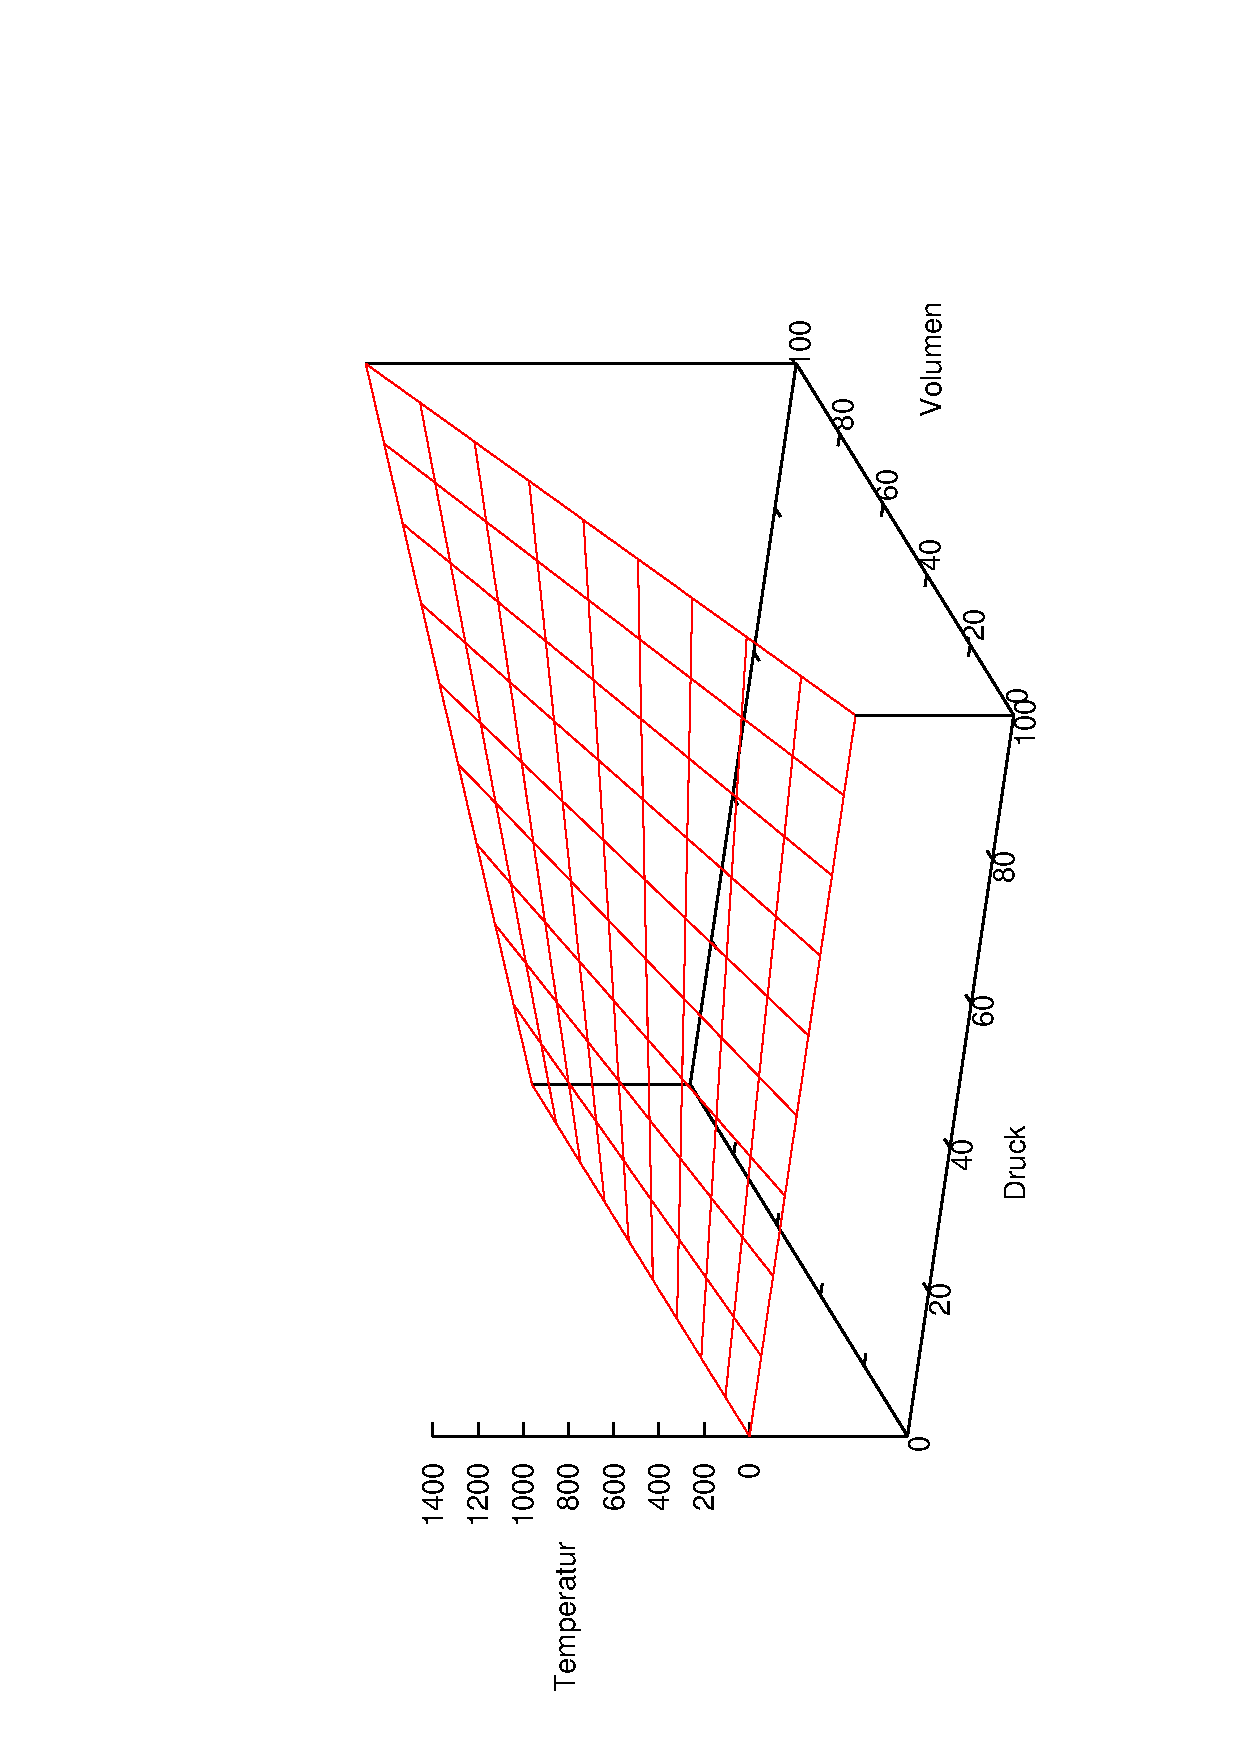
\includegraphics[width=0.34\textwidth,angle=-90]{bilder/gasB1}}  
\subfigure[Volumen gegen Druck (vorne) und Temperatur
   (rechts)]{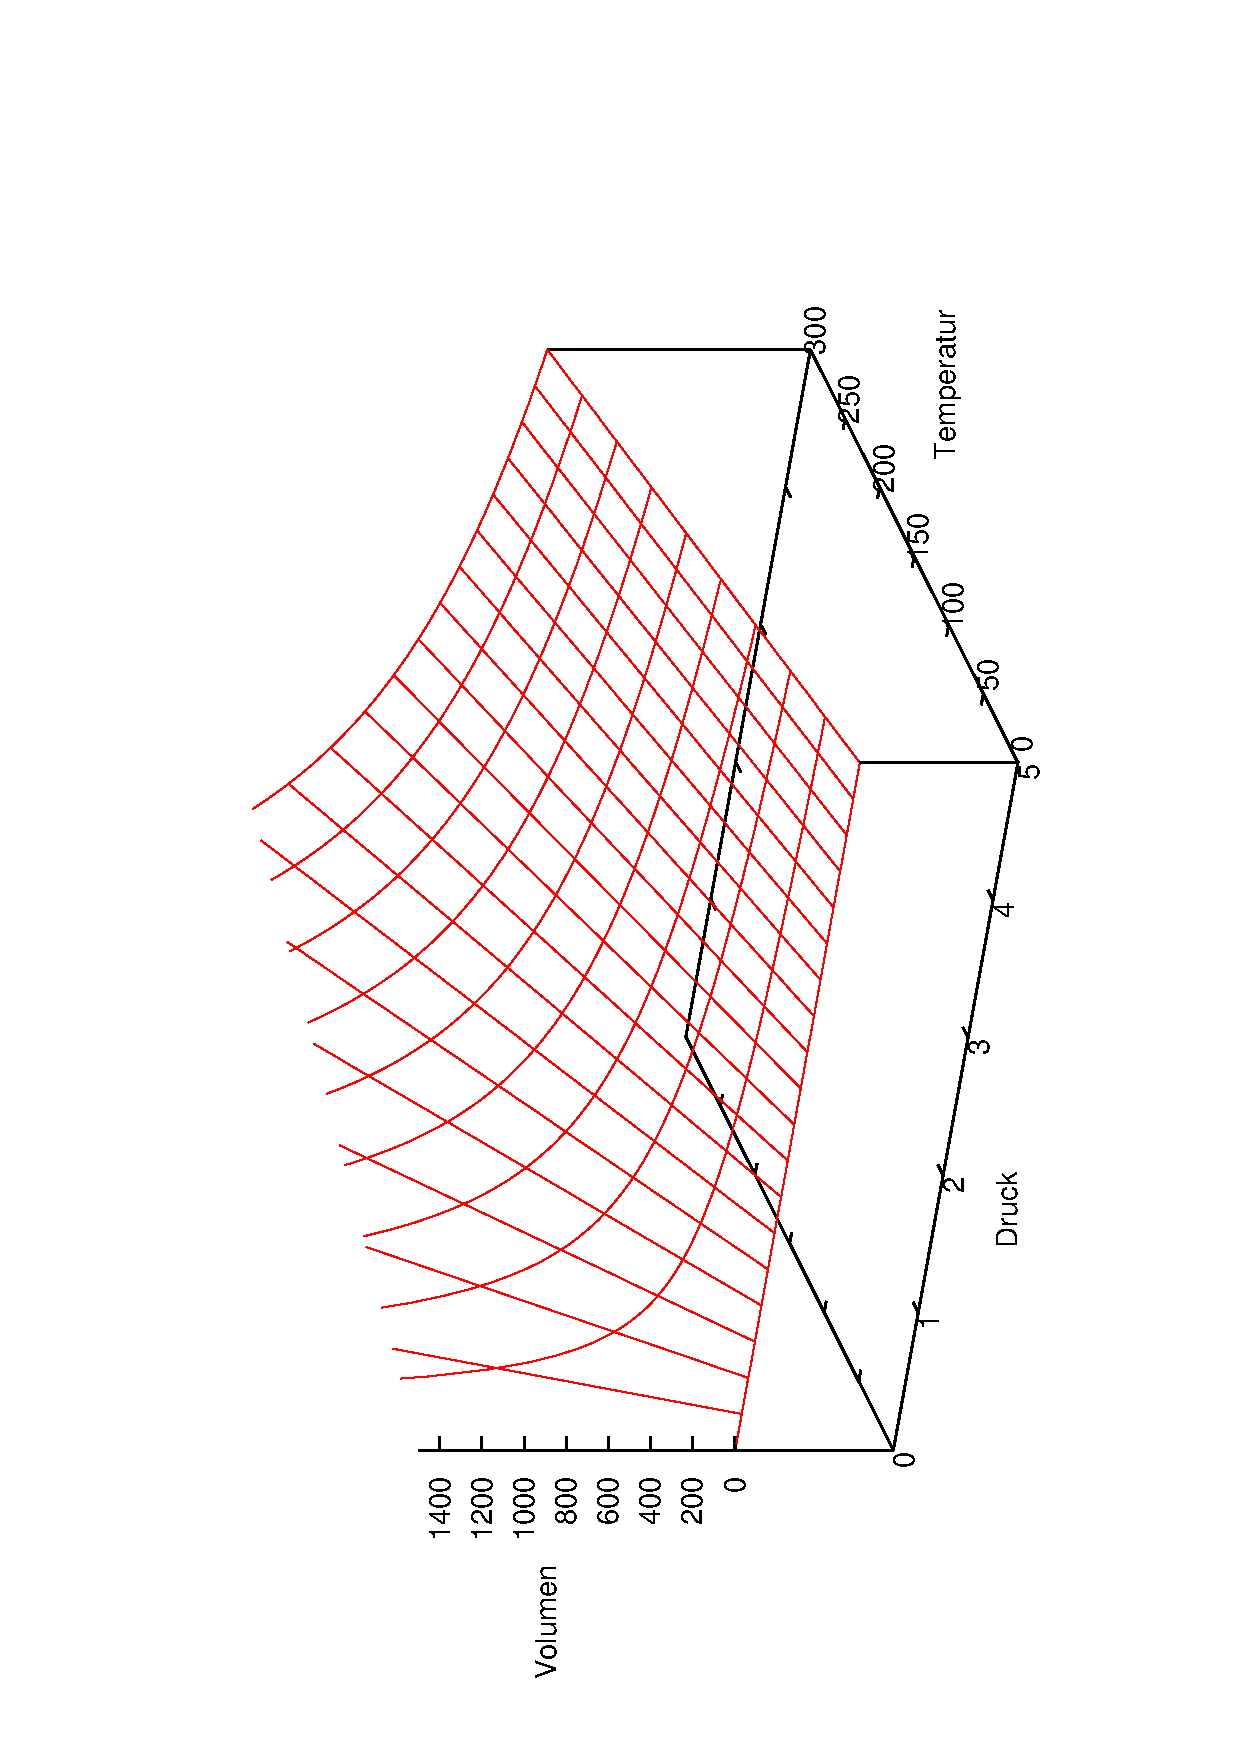
\includegraphics[width=0.34\textwidth,angle=-90]{bilder/gasB2}}
\caption[Flächen der Idealen Gasgleichung]{Fl"ache der Idealen
     Gasgleichung im $\mathbb R^3$ -- Zahlen gelten für $1
     \operatorname{mol}$ Gas. Die eingezeichneten Linien sind Isobare,
     Isotherme bzw. Isochore.}
   \label{abb_ideale-gasgleichung}
\end{figure}

Wir unterscheiden folgende entscheidende F"alle:
\begin{center}
   \begin{tabular}[c]{l l l}
   Isotherm & konstante Temperatur & $\diff T = 0$\\
   Iosbar & konstanter Druck & $\diff p = 0$\\
   Isochor & konstantes Volumen & $\diff V = 0$\\
   Adiabatisch & kein W"armeaustausch & $\diff Q = 0$
\end{tabular}
\end{center}
 Sie sind spezialf"alle
f"ur den \emph{Ersten Hauptsatz der Thermodynamik} (s.
\ref{kap_erste-hauptsatz-thermodynamik}) und k"onenn mit
diesem genauer betrachtet werden. 

\subsection{Isotherm}
\label{kap_isotherm}

Es gilt
$$
T = T_0 = const \text{ oder } {\diff T= 0}
$$
und mit \eqref{eqn_ideale-gasgleichung} folgt 
$$
p \sim \frac{1}{V}
$$
Im Experiment muss das Gas \emph{langsam} komprimiert werden, damit
die entstehende W"arme komplett in ein W"armebad (mit $T = T_0$)
abgegeben werden kann.

Die \textbf{Isotherme \index{Isotherme
    Kompressibilit"at}\index{Kompressibilit"at}Kompressibilit"at}\footnote{Die
Kompressibilit"at $\kappa$ ist uns noch aus
Kap. \ref{kap_krafte-auf-festkorper} bekannt. Dieses $\kappa$ hier ist
der Kehrwert eines \emph{Kompressionsmoduls} ($\kappa = \frac{1}{K}$)
und hat mit dem \emph{Adiabatenkoeffizient} $\kappa$ wenig zu tun.}
\begin{equation}
   \label{eqn_Isotherme-kompressibilit"at}
   \kappa = - \frac{1}{V} \left ( \frac{\partial V}{\partial p} \right )_T
\end{equation}
gibt die relative Volumen"anderung bei konstanter Temperatur pro
Druck"anderung an.

Wie wir schon gesehen haben (in \eqref{eqn_thermische-energie}) h"angt
$U$ alleine von der Temperatur $T$ ab. Ist diese konstant, wie in
diesem Fall, folgt aus $\diff T = 0$ auch $\diff U = 0$.  Weiter folgt mit
\eqref{eqn_erster-hauptsatz-ideales-gas}:
\begin{equation}
   \label{eqn_isotherm_unnere-energie}
   -\diff W = \diff Q = p \cdot \diff V = \frac{nRT}{V}\diff V
\end{equation}
\begin{Wichtig}
Es wird also die komplette, dem System zugef"ugte Energie $\Delta Q$ in
\emph{Volumenarbeit} umgewandelt.   
\end{Wichtig}
%
%
Durch Integration kann man einfach die \emph{Energie} ausrechnen, die
ein Gas verrichtet, welches sich isotherm von $V_1$ auf $V_2$
ausdehnt:
\begin{equation}
   \label{eq:3}
W = - nRT \int_{ V_1 }^{ V_2 } \frac{1}{V}\diff V = nRT \ln \frac{V_1}{V_2}   
\end{equation}




Mit \eqref{eqn_ideale-gasgleichung} folgt schlie"slich noch
\begin{equation}
%   \label{eq:5}
   pV = nRT = const ~\Rightarrow ~ p \sim \frac{1}{V}
\end{equation}
Man spricht hier vom \textbf{\textsc{Boyle}-\textsc{Mariotte}'schen Gesetz}.




\subsection{Isobar}
\label{kap_isobar}

Es gilt
$$
p = p_0 = const \text{ oder } { \diff p = 0}
$$
Und mit \eqref{eqn_ideale-gasgleichung} folgt
$$
V \sim T
$$

Der \textbf{isobare \index{isobarer
Ausdehnungskoeffizient}Ausdehnungskoeffizient}
\begin{equation}
   \label{eqn_isobarer-ausdehnungskoeffizient}
   \gamma_v = \frac{1}{V} \left ( \frac{\partial V}{\partial T }
   \right )_p
\end{equation}
gibt die relative Volumenausdehnung pro Kelvin Temperaturerh"ohung an,
wenn $p = const$.


F"ur ein konstantes $p$ erhalten wir $\diff p = 0$. Nun f"uhren wir (vorl"aufig)
ein:
\begin{Def}
   [\index{Enthalpie}Enthalpie]
Die Enthalpie $H$ ist
\begin{equation}
   \label{eqn_entropie}
   H = U + p \cdot V 
\end{equation}
Sie besteht also aus \emph{Innerer Energie} und
\emph{Volumenarbeit}. Man verwendet $H$, um die \emph{Energie} im
System anzugeben.
\end{Def}

Es gilt nun also f"ur $\diff H$, wenn man
\eqref{eqn_erster-hauptsatz-ideales-gas} einsetzt (und $\diff p = 0$
wegen isobar beachtet):
$$
\diff H = \diff U + V \diff p + p \diff V = \diff Q + V \diff p
$$
und damit
\begin{equation}
   \label{eq:4}
   \diff H = \diff U + p \diff V = \diff Q
\end{equation}
\begin{Wichtig}
   Es wird die komplette zugef"uhrte W"armemenge in Enthalpie imgewandelt.
\end{Wichtig}
Wir k"onnen dies verwenden, um die Spezifische W"arkekapazit"at $C_p$
umzuschreiben; \emph{bei konstantem Druck} gilt:
\begin{equation}
   \label{eqn_Cp}
   C_p = \left ( \frac{\partial H }{\partial T} \right )_p
\end{equation}
Vergleiche Gl. \eqref{eqn_Cv}.






\subsection{Isochore}
\label{kap_isochore}

Es ist 
$$
V = V_0 = const \text{ oder } { \diff V = 0}
$$
 und mit \eqref{eqn_ideale-gasgleichung}
folgt
$$p \sim T$$
Der \textbf{Isochore \index{ioscorer Spannungskoeffizient}Spannungskoeffizient}
\begin{equation}
   \label{eqn_ioscorer-spannungskoeffizient}
   \gamma_p = \frac{1}{p} \left ( \frac{\partial p}{\partial T} \right )_V
\end{equation}
gibt an, wie sich der Druck bei konstantem Volumen vergr"o"sert, wenn
die Temperatur ge"andert wird.

Mit Gl. \eqref{eqn_erster-hauptsatz-ideales-gas} und $\diff V = 0$
gilt
\begin{equation}
   \label{eqn_waerme-aus-waermekapazitaet}
   \diff Q = \diff U = C_V \cdot \diff T
\end{equation}
\begin{Wichtig}
D.h. die zugef"uhrte W"armemenge wird \emph{vollst"andig} in innere
Energie umgesetzt.    
\end{Wichtig}
Hier kann man jetzt definieren:
\begin{equation}
   \label{eqn_Cv}
   C_V = \left ( \frac{\partial U}{\partial T} \right )_V
\end{equation}
Vgl. Gl. \eqref{eqn_Cp}.



% \subsection{Volumen"anderung}
\subsection{Zusammenhang zwischen den Koeffizienten}
\label{kap_zusammenhang-zwischen-den-koeffizienten}
\label{kap_volumenanderung}

Die komplette Volumen"anderung eines Volumens $V(p,T) = V_0$ schlie"slich
ergibt sich bei einer "Anderung von $T$ und $p$ mit
\eqref{eqn_Isotherme-kompressibilit"at}  und
\eqref{eqn_isobarer-ausdehnungskoeffizient} zu
$$
\diff V = \left ( \frac{\partial V}{\partial p} \right )_T \diff p +
\left ( \frac{\partial V}{\partial T } \right )_p \diff T =
- \kappa \cdot V_0 \cdot \diff p + \gamma_V \cdot V_0 \cdot \diff T
$$
Bei isochoren Prozessen bleibt das Volumen konstant ($\diff V = 0$) und
man bekommt hierf"ur
$$
\kappa \cdot \diff p = \gamma_V \diff T
$$
%
%
Und so erh"alt man durch Division durch $\diff T$ und mit
Gl. \eqref{eqn_ioscorer-spannungskoeffizient} schlie"slich als
Zusammenhang zwischen den Koeffizienten:
\begin{equation}
   \label{eqn_zshg-koeffizienten}
   \kappa \cdot \gamma_p \cdot p = \gamma_V 
\end{equation}




\subsection{Adiabate}
\label{kap_adiabate}

Es findet \emph{kein W"armeaustausch} mit der Umgebung statt; also
ist 
$$
Q = Q_0 = const \text{ oder } {\diff Q = 0}
$$
In der Natur finden solche Vorg"ange h"aufig als \emph{Grenzf"alle}
statt; wenn sich der Zustand eines Gases so schnell "andert, dass das
Gas einfach keine Zeit hat, mit der Umgebung W"arme auszutauschen --
bzw. nur vernachl"assigbar wenig.

F"ur den 1. HS \eqref{eqn_erster-hauptsatz-ideales-gas} folgt (mit
\ref{eqn_Cv}) da $\diff Q = 0$:
\begin{equation}
   \label{eq:1}
   \diff U = - p \diff V = C_V \diff T
\end{equation}
Verwenden wir nun noch \eqref{eqn_ideale-gasgleichung} und ersetzen $p
= \frac{nRT}{V}$ und nach \eqref{eqn_c_v} $C_V = \frac{f}{2} K_BN$ so
gilt (nach anschlie"sender Integration):
\begin{eqnarray}
\nonumber
\frac{f}{2} K_B N \diff T &=& - \frac{NK_BT}{V} \diff V   \\
\nonumber
\frac{f}{2}  \cdot \frac{1}{T} \diff T &=& -   \frac{1}{V}
\diff V   \\
\nonumber
\frac{f}{2}  \int \frac{1}{T} \diff T &=& - \int \frac{1}{V}
\diff V  \\
\nonumber
\frac{f}{2} \ln T &=& - \ln V + \const \\
\nonumber
\ln (  T^{ \frac{f}{2} } \cdot V ) &=& \const \\
\label{eq:7}
T^{ \frac{f}{2} } \cdot V  &=& \const 
\end{eqnarray}
Die Gleichung kann man noch mit $K_BN$ potenzieren und erh"alt unter
Beachtung von \eqref{eqn_differenz-c}:
\begin{equation}
   \label{eq:6}
   T^{ C_V } \cdot V^{ (C_P - C_V) }  = \boxed {T\cdot V^{ \kappa - 1
     }= const }
\end{equation}
Alternativ kann man aus \eqref{eq:7} mit \eqref{eqn_ideale-gasgleichung} $T$
ersetzen
(und ein paar Konstanten k"urzen). Beachtet man nun, dass $V\cdot V^{
  \frac{2}{f}} = V^{ \frac{2+f}{f} }$ ist und verwendet
\eqref{eqn_adiabatenkoeffizient} statt $\frac{2+f}{f}$, so erh"alt man
\begin{equation}
   \label{eq:9}
\boxed{
   pV^\kappa = const
}
\end{equation}
(Dieses Ergebnis h"atte man auch erhalten, h"atte man mit
\eqref{eqn_ideale-gasgleichung} das $TV^{\kappa-1 } =
\frac{T}{V}V^\kappa$ das $\frac{T}{V}$ ersetzen k"onnen.)




\subsection{Erw"armung bei adiabatischer Kompression}
\label{kap_erwarmung-bei-adiabatischer-kompression}

F"ur isotherme Prozesse gilt $pV = const$ und f"ur adiabatsiche
$pV^\kappa = const$. (In einem $V$-$p$-Diagramm\footnote{also $p$ auf
  der $x$-Achse und $V$ auf der $y$-Achse} sind die Isothermen steiler
als die Adiabaten.) Es liegt also nahe, diese beiden Prozesse zu
vergleichen. Siehe dazu Abb. \ref{abb_isotherm-adiabatisch}: Die
Adiabate schneidet die beiden Isothermen an zwei Stellen. Bei
adiabatischer Kompression -- also wenn wir einer Adiabaten folgen --
wechseln wir folglich von der niedrigen auf die h"ohere Isothermen und
folglich muss sich die Temperatur bei der Kompression erh"ohen.

Das kommt daher, dass bei der Kompression mechanische Arbeit in W"arme
umgewandelt wird. Beim isothermen Prozess ist es nun so, dass diese
W"arme abgegeben werden kann, beim adiabatischen dagegen verbleibt
diese W"arme im Gas und sorgt hier daf"ur, dass die Temperatur steigt.

% \begin{figure}
%    \centering
% 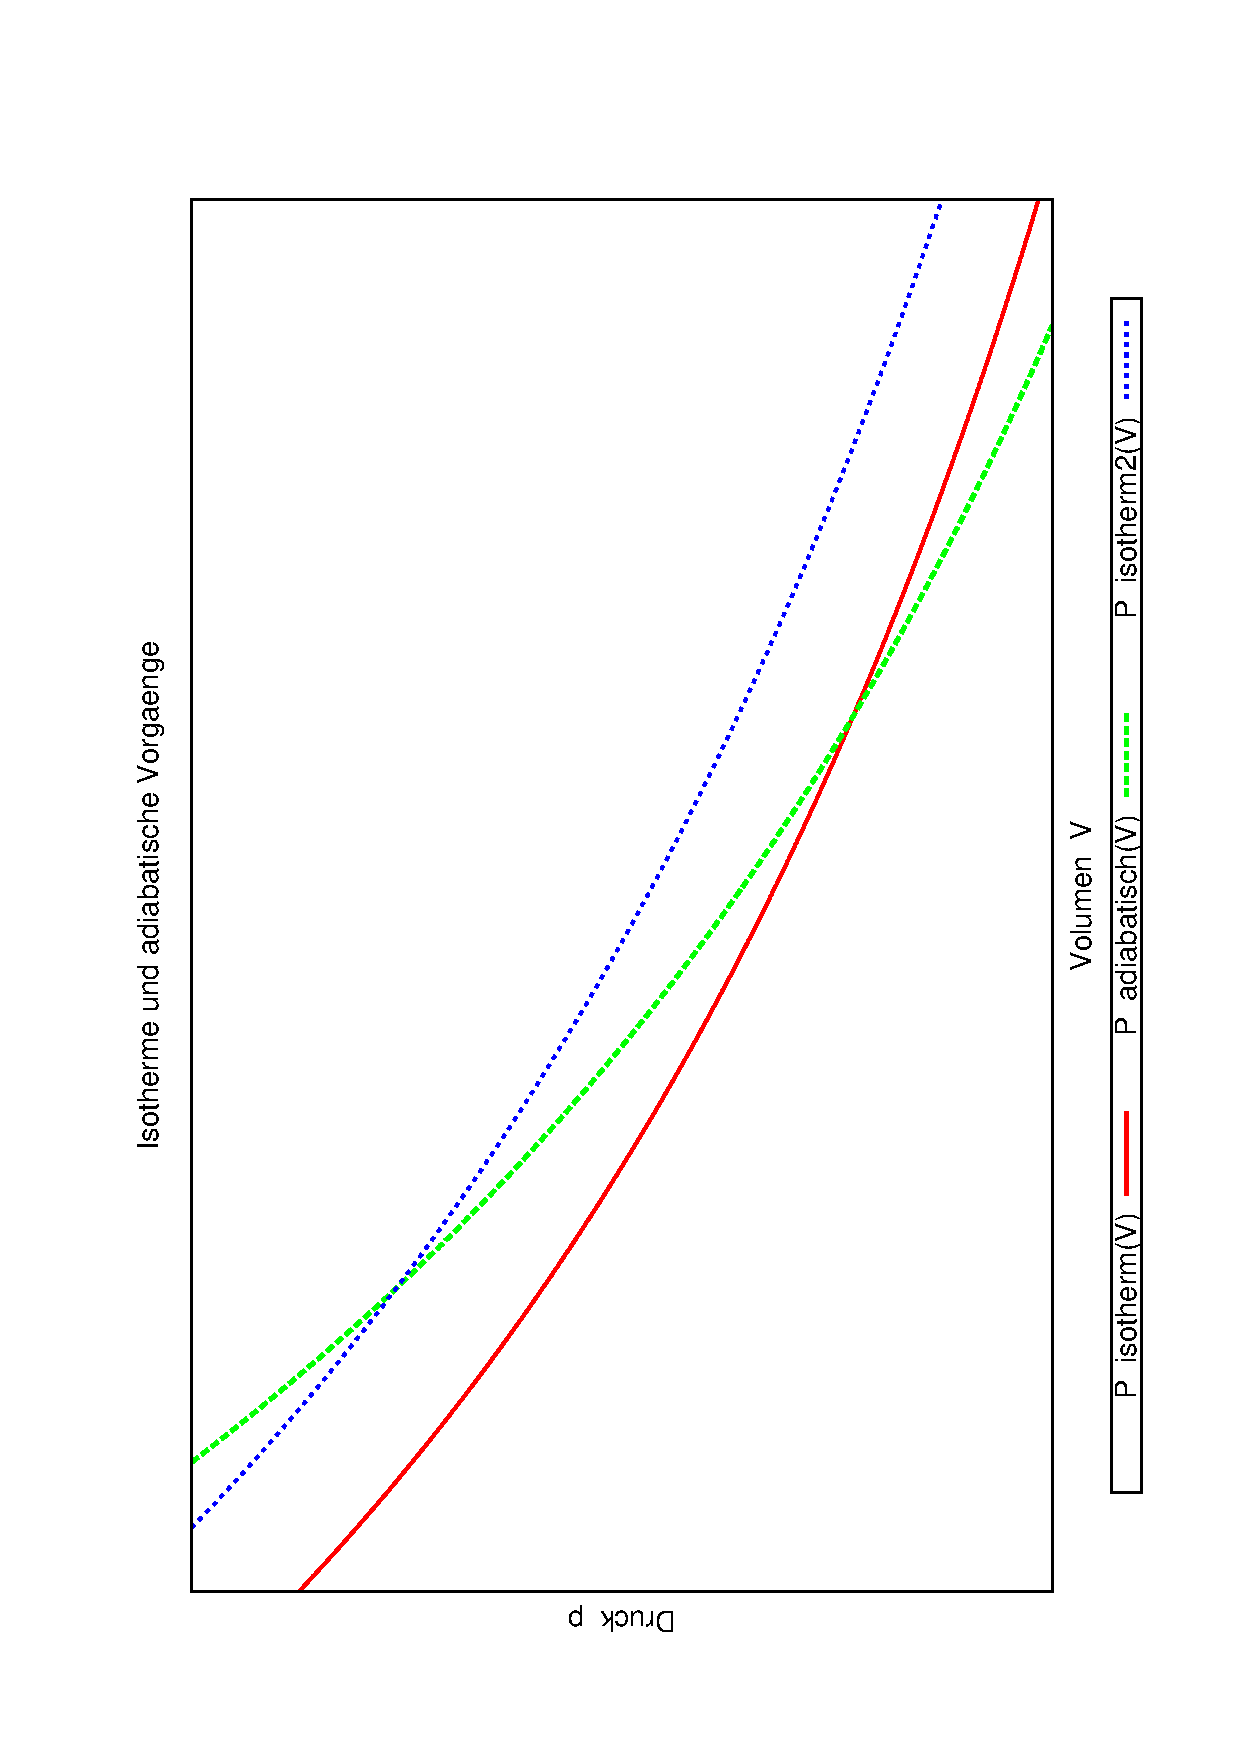
\includegraphics[width=0.5\textwidth,angle=-90]{bilder/iso-adiab}
%    \caption{Abbildung eines adiabatischen und zweier Isothermer Prozesse}
%    \label{abb_isotherm-adiabatisch}
% \end{figure}












\section{Zweiter Hauptsatz}
\label{kap_zweiter-hauptsatz}

W"arend der erste Hauptsatz noch die Energieerhaltung postuliert,
beschreibt der zweite Hauptsatz, \emph{wie} sich die Energieformen
ineinander umwandeln k"onnen.

Wir f"uhren dazu die Entropie ein:

\begin{Def}
   [\index{Entropie}Entropie]
Die Entropie $S$ ist eine Zustandsgr"o"se, die zunimmt, wenn sich ein
System einem Gleichgewichtszustand ann"ahrt. 
\end{Def}
Es gilt 
%bei \emph{reversiblen} Prozessen (mit
%\eqref{eqn_erster-hauptsatz} und der Idealen-Gas-Gleichung):
dabei mit der reversiblen W"armemenge:
\begin{equation}
   \label{eqn_def_entropie}
   \diff S = \frac{\diff Q_\text{rev}}{T} 
% =
%  \frac{\diff U + p \diff V}{T}
% =
% \frac{\frac{f}{2} N K_B  \diff T}{T} + \frac{N K_B \diff V}{V}
\end{equation}

Eigentlich setzt sich $\diff S$ zusammen aus einem
\emph{Entropiefluss} $\diff S^\text{e}$ von Au"sen in das System und
einer inneren \emph{Entropieproduktion} $\diff S^\text{i}$ durch
Prozesse im Inneren des Systems:
\begin{equation}
 \diff S = \diff S ^\text{e} + \diff S^\text{i}
\end{equation}
Analog zu Gl. \eqref{eqn_def_entropie} k"onnte man schreiben:
\begin{equation*}
   \diff S^\text{e} = \frac{\diff Q}{T}
\end{equation*}
wobei diesmal $\diff Q$ die gesamte mit der Umgebung ausgetauschte
W"armemenge ist. 

Mit der Definition folgt:
\begin{description}[\setlabelstyle{\bfseries\slshape}]
\item[$\Delta S > 0$] \index{irreversibler}irreversibler Prozess
\item[$\Delta S = 0$] \index{reversibler}reversibler Prozess
\item[$\Delta S < 0$] Wird in der Natur nicht beobachtet (zumindest
   nicht in \emph{makroskopischen} Systemen.
\end{description}
Die W"armemenge
\begin{equation*}
   \Delta Q = T \cdot \Delta S
\end{equation*}
die bei einem Prozess frei wird, bezeichnet man auch als
\emph{\index{Abw"arme}Abw"arme} oder
\emph{\index{Verlust-Energie}Verlust-Energie}, weil sie bei dem
Prozess nur zur "Anderung der Entropie verwendet wird, nicht aber, um
wirklich Arbeit zu verrichten.

Wir k"onnen sagen, dass die Entropie die \textbf{Zahl der Zust"ande}
eines Systems ist. F"uhrt man in diesem System eine
\index{Zwangsbedingung}Zwangsbedingung ein, so reduziert man die
m"ogliche Zahl der Zust"ande und \emph{erniedrigt} damit die
Entropie. Um das System auf diese Zwangsbedingungen zu bringen, sind
aber Zwangs\emph{kr"afte} n"otig. Man muss Arbeit investieren, um das
System in den neuen, mit den Zwangsbedingungen vertr"aglichen Zustand
zu bringen.

\begin{Beispiel}
   Bei dem ber"uhmten Beispiel eines Kastens der zur H"alfte mit Gas
   gef"ullt ist, haben wir die Zangsbedingung der Trennung. Wird die
   Trennung weggenommen -- also die Zwangsbedingung aufgehoben --
   verteilt das Gas sich im ganzen, ihm zur Verf"ugung stehenden Raum,
   und maximiert so seine Entropie. M"ochte man den urspr"unglichen
   Zustand wieder herstellen, so muss man \emph{von Au"sen} Energie
   investieren, um die Teilchen wieder zur"uckzusortieren.
\end{Beispiel}


Ebenso kann man die Entropie als \textbf{Informationsgehalt}
verstehen: Je gr"o"ser die Information, desto kleiner die Entropie. 
\begin{Beispiel}
   In dem halbvollen Kasten ist der Informationsgehalt h"oher: Man kann
   mit absoluter Sicherheit f"ur jedes Teilchen einen Punkt
   "`irgendwo"' innerhalb von $\frac{1}{2}V$ annehmen. Bei dem gro"sen
   Kasten dagegen kann man f"ur die Teilchen nur noch sagen, sie
   befinden sich "`irgendwo"' in $V$. Der Informationsgehalt hat also
   vom halbvollen zum vollen Kasten so \emph{ab}genommen, wie die
   Entropie \emph{zu}genommen hat.
\end{Beispiel}

Nicht ganz korrekt, aber daf"ur anschaulich, kann
man sagen, dass die Entropie ein \emph{Ma"s f"ur die Unordnung} eines
Systems ist.

\abs 
Wie wir in Kap. \ref{kap_reversible-und-irreversible-prozesse}
sehen werden, strebt die Natur zu einem \emph{Gleichgewicht}; sie ist
also bestrebt, dass $\Delta S > 0$ ist. Man k"onnte also sagen, sie
ist bestrebt, die Entropie zu maximieren.

So ist auch der zweite Hauptsatz zu verstehen:
\begin{Wichtig}
   [\index{Zweiter Hauptsatz der Thermodynamik}Zweiter
   \index{Hauptsatz Thermodynamik}Hauptsatz der Thermodynamik]
In einem abgeschlossenen (adiabatischen) System kann die Entropie
nicht ab-, sondern nur zunehmen, und bleibt h"ochstens bei reversiblen
Prozessen konstant:
\begin{equation}
   \label{eqn_zwetier-hauptsatz}
   \boxed{
\Delta S \geq 0
}
\end{equation}
\end{Wichtig}
Man kann ihn auch umformulieren:
\begin{quote}
   W"arme flie"st von selbst nur von w"armeren zu k"alteren Stellen --
   niemals umgekehrt
\end{quote}

Interessant ist noch, dass bei einem irreversibel ablaufenden,
adiabatischen Prozess Entropie $\diff S^\text{i}$ im System erzeugt
wird, bei einem reversiblen logischerweise nicht; Entropie"anderung
(\emph{-fluss} $\diff S^\text{e}$) von au"sen wird aber in keinem der
F"alle ins System gebracht.

% Wiki: Adiabatische_Zustands"anderung






\section{Dritter Hauptsatz}
\label{kap_dritter-hauptsatz}

Der Dritter Hauptsatz ist sehr schlicht:
\begin{Wichtig}
   [Dritter \index{Hauptsatz Thermodynamik}Hauptsatz der \index{Dritter Hauptsatz der
     Thermodynamik}Thermodynamik]
Es ist nicht m"oglich, ein System bis auf $T =0$ abzuk"uhlen.
\end{Wichtig}
Au"serdem gilt f"ur die Entropie:
$$
S(T,p,V) \stackrel{T \to 0}{\to} S_0
$$
d.h. wenn $T$ verschwindet, so geht $S$ unabh"angig von den anderen
Parametern $p$, $V$, ... gegen den Zustand $S_0$ wobei f"ur diesen
gilt:
$$
S_0 =K_B \ln \Omega_0 
$$
wobei $\Omega_0$ die Anzahl m"oglicher Mikrozust"ande im System
darstellt.

F"ur alle physikalisch-chemischen Reaktionen, bei denen die
teilnehmenden Stoffe am absoluten Nullpunkt als ideale kristalline
Festk"orper vorliegen, gilt:
$$
S_0 = 0
$$
und damit folgt $ln \Omega_0 = 0$ bzw. $\Omega_0 = 1$. Es gibt also
nur einen einzigen Zustand, den das System am absoluten Nullpunkt
einnehmen kann.









\section{Freie Energie und Enthalpie}



\subsection{Freie Energie}
\label{kap_freie-energie}



In der \emph{Mechanik} versuchen (makroskopische) K"orper ihre
(potentielle) Energie zu minimieren: Ein K"orper f"allt so weit er kann
nach "`unten"', damit die potentielle Energie m"oglichst klein wird. In
der \emph{Thermodynamik} ist dies offensichtlich nicht so -- sonst
w"urden sich alle Luftteilchen m"oglichst nahe "uber dem Boden befinden
und weiter oben g"abe es keine Luft mehr.

Um diesen Drang der Natur nach einem Energieminimum weiterhin als
physikalische Regel beibehalten zu k"onnen, m"ussen wir eine Art
\emph{thermodynamisches Potential} definieren:

\begin{Def}
   [\index{Freie Energie}Freie Energie $\mathcal F$]
Die Freie Energie $\mathbf \mathcal{F}$ ist definiert als
\begin{equation}
   \label{eqn_freie-energie}
\boxed{
  \mathcal F = U - T \cdot S
}
\end{equation}
mit der Entropie $S$ und der Inneren Energie $U$.  

Wir bezeichnen $\mathcal F$ auch als \textbf{\index{Thermodynamisches
    Potential}thermodynamisches Potential}.
\end{Def}
%
Im Gegensatz zur freien Energie, bezeichet man als \textbf{gebundene
  Energie}:
\begin{equation}
   \label{eqn_gebundene-energie}
 TS =    U - \mathcal F
\end{equation}
\begin{Wichtig}
   [Freies \index{Freies Energieminimum}Energieminimum] Die Natur ist
   (bei konstantem Volumen -- also bei einem \emph{mechanisch
     isolierten} System -- und konstanter Temperatur) bestrebt, dass
   die \textbf{freie Energie $\mathcal F$ minimal} wird. Dies
   entspricht dem Gleichgewichtszustand.
\end{Wichtig}

Vergleichen wir das mit dem zweiten Hauptsatz der Thermodynamik
(Kap. \ref{kap_zweiter-hauptsatz}), der besagt, dass $S$ maximal
werden soll, sehen wir, dass diese beiden in Einklang stehen: Wird $S$
gr"o"ser, so wird $\mathcal F$ wegen des Minuszeichens in
\eqref{eqn_freie-energie} kleiner.

% Betrachten wir nun isotherme Zustands"anderungen (bei denen also
% $\diff T = 0$ und mit Gl. \eqref{eqn_thermische-energie} auch $\diff
% U = 0$) ist, so gilt

\begin{Wichtig}
   Es wird sich stets ein Gleichgewicht -- bzw. ein \emph{Kompromiss}
   zwischen der Maximierung von $S$ und der Minimierung von $\mathcal
   F$ geben.\footnote{Mimimierung von $\mathcal F$: Gasteilchen
     bewegen sich nicht mehr uns liegen am Boden ($\mathcal F$ min \Ipl $N\bar
     u$ min \Ipl $\bar u$ min \Ipl $\bar v$ min)\\Maximierung von $S$:
     Teilchen verteilen sich homogen; nehem m"oglichst viel Platz
     ein.}  Dieser Kompromiss ist die \textsc{Boltzmann}-Verteilung
   (Kap.  \ref{kap_exkurs:bolzmann-faktorn-und-thermische-energie}).
\end{Wichtig}





\subsection{Freie Enthalpie}
\label{kap_freie-enthalpie}

Analog zur Freie Energie definiert man in einem Sysem f"ur die Enthalpie:
\begin{Def}
   [Freie Enthalpie $G$] 
   \begin{equation}
      \label{eq:207}
      G = H - TS
   \end{equation}
Es handelt sich dabei um ein weiteres \textbf{\index{Thermodynamisches
  Potential}Thermodynamisches Potential}
\end{Def}



\begin{Wichtig}
   [\index{Freies Enthalpieminimum}Freies Enthalpieminimum] Bleiben
   Druck und Temperatur eines Systems konstant, ist die Natur
   bestrebt $G$ zu minimieren.
\end{Wichtig}
Dieser Satz wird h"aufig in der Chemie gebraucht, weil hier die meisten
Reaktionen bei (konstantem) Druck ablaufen (in offenen Gef"a"sen). Man
sieht hier: Eine Reaktion l"auft nur dann ab, wenn $\Delta G < 0$
ist. Der Chemiker bezeichnet dies als \emph{exergonische}
Reaktion. Im Gegensatz dazu ben"otigen \emph{endergonische} Reaktionen
mit $\Delta G > 0$ \emph{Energiezufuhr}.









\section{Kreisprozesse}
\label{kap_kreisprozesse}

\begin{Def}
   [\index{Kreisprozess}Kreisprozess] Ein thermodynamisches System
   durchl"auft verschiedene Zust"ande, kommt anschlie"send aber wieder
   zum Ausgangszustand zur"uck: Es hat wieder die selben
   Zustandsgr"o"sen.
\end{Def}

Bei einem Kreisprozess bleibt die Innere Energie $U$ \emph{zwischen
  Anfangs- und Endzustand} erhalten: $U_a = U_e$ bzw. $\Delta U = 0$
(wobei sich das "`$\Delta $"' auf dem gesamten Prozess bezieht). Mit
dem ersten HS \eqref{eqn_erster-hauptsatz} folgt so:
$$
 \Delta Q = - \Delta W
$$
Es wird also alle aufgenommene W"arme direkt in Arbeit umgesetzt (und
anders herum). Das "`$-$"' bedeutet hier, dass wenn man W"arme in das
System hineinsteckt, man Arbeit verrichtet bekommt, und anderst herum
eine W"armemenge erh"alt, wenn man an dem System Arbeit verrichtet. Wir
bezeichnen solche Systeme auch als
\textbf{\index{W"armekraftmaschinen}W"armekraftmaschinen}. Sie k"onnen
(nur) arbeiten, wenn ihnen st"andig W"arme zugef"uhrt wird.


\subsection{Reversible und Irreversible Prozesse}
\label{kap_reversible-und-irreversible-prozesse}

Wir unterscheiden bei Kreisprozessen, ob ein Prozess re- oder
irreversibel ist. Kann er in beiden Richtungen ablaufen, so hei"st er
\emph{reversibel}, kann er nur in einer Richtung ablaufen, so ist er
\emph{irreversibel}. In der Natur kommen erstere h"ochstens auf der
mikroskopischen Scala vor -- im makroskopischen Bereich bleiben
reversible Prozesse leider Gedankenexperimente.
\begin{Wichtig}
   Thermodynamische Prozesse laufen h"aufig nur in eine Richtung von
   selbst ab.
\end{Wichtig}

\begin{Beispiel}
   Haben wir bspw einen Kolben, dessen Innendruck den Au"sendruck
   "ubersteigt, so wird der Kolben herausgeschoben und verrichtet so
   Arbeit. Der Umgekehrte Fall ist zwar nach dem ersten Hauptsatz der
   Thermodynamik m"oglich, wird in der Natur jedoch nicht eintreten.
\end{Beispiel}


Eine gute Erkl"arung daf"ur ist, dass der ausgedehnte Kolben ein
\emph{Gleichgewichtszustand} ist. Die Natur ist bestrebt, diesen
Gleichgewichtszustand einzustellen -- jedoch alles andre als bestrebt,
diesen wieder zu verlassen; der Prozess ist also folglich
\emph{irreversibel}. Dies motiviert den zweiten Haupsatz
(Kap. \ref{kap_zweiter-hauptsatz}).







\subsection{Der \textsc{Carnot}-Prozess}
\label{kap_carnot-prozess}

Es handelt sich hierbei um einen \emph{fundamentalen
  Kreisprozess}, in dem die vier Zust"ande A bis D periodisch
durchlaufen werden. Wir betrachten 
\begin{itemize}
\item einen Gasbeh"alter mit Kolben, in dem das Gas
   ("`\textbf{Arbeitsgas}"') komprimiert bzw. expandiert wird.
\item Der Beh"alter wird abwechselnd in W"armeb"ader unterschiedlicher
   Tempetarturen getaucht: $T_w$ f"ur warme und $T_k$ f"ur kalte B"ader.
\end{itemize}


\begin{figure}
   \centering
   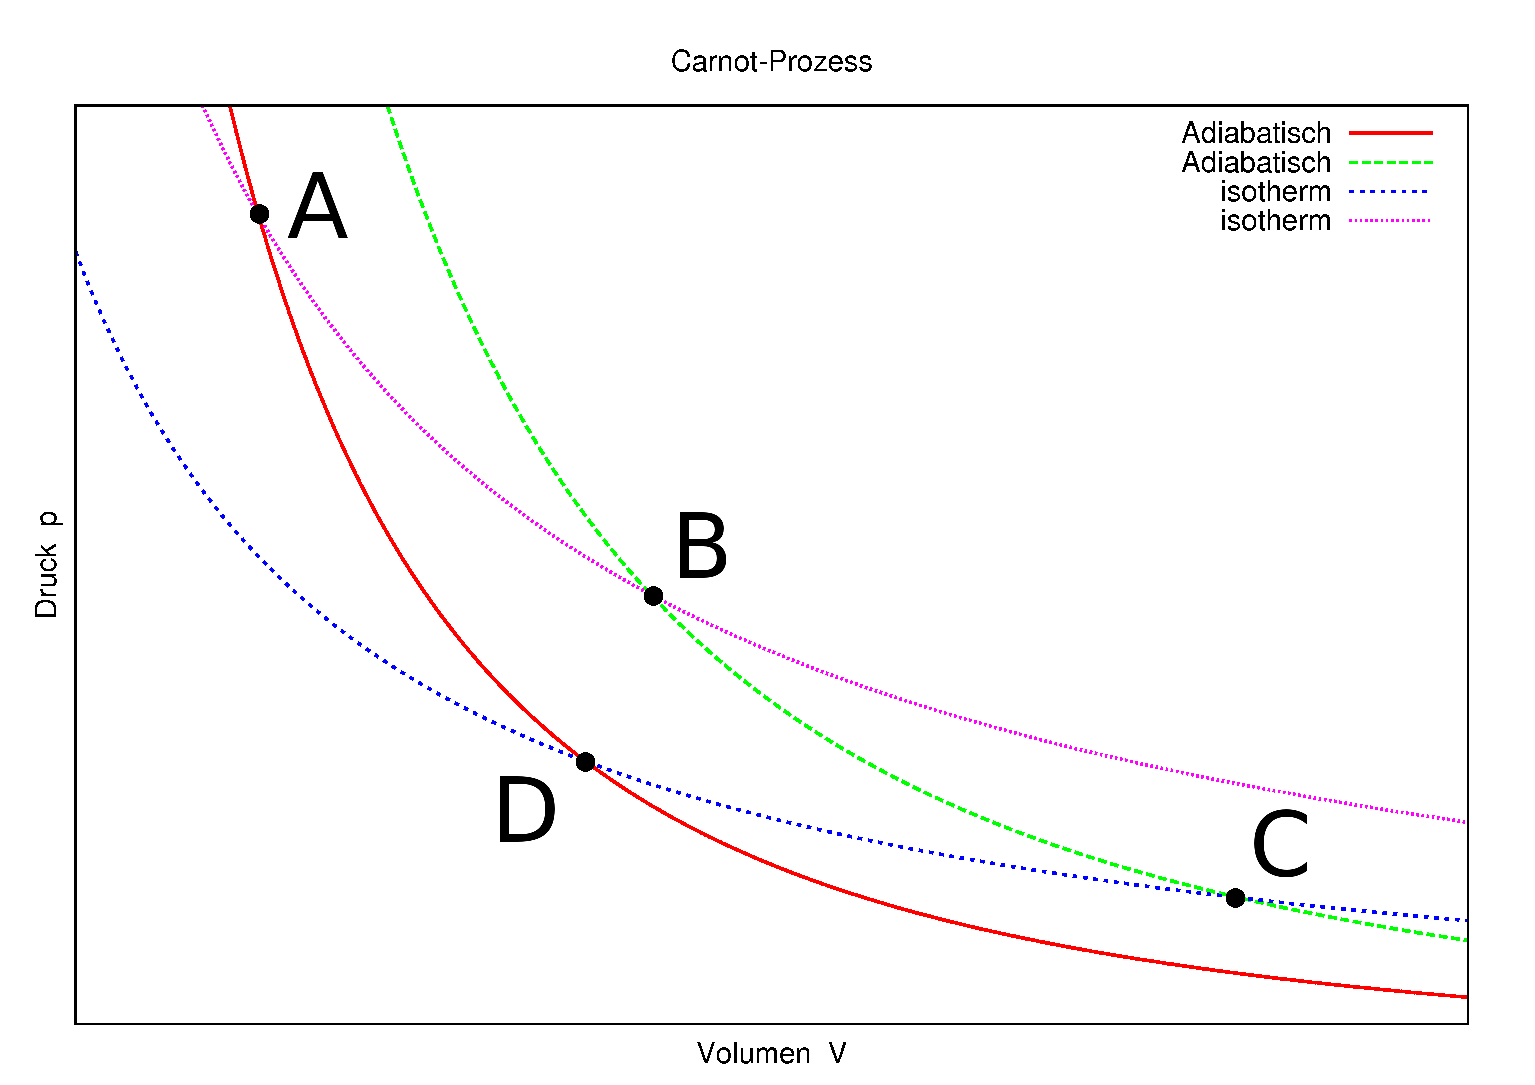
\includegraphics[width=0.7\textwidth]{bilder/carnot1_mod1}
   \caption[Phasendiagramm: Carnot-Prozess]{$p$-$V$-Diagramm des
     Carnot-Prozesses. Die beiden steilen Kurven geh"oren zu
     Adiabatischen Vorg"angen, die flachen zu isothermen. Verwendet
     man ein $V$-$p$-Diagramm tauschen Adiabaten und Isothermen die
     Position.}
   \label{abb_carnot-prozess}
   \label{abb_isotherm-adiabatisch}
% Das Zweite Label ist da, um eine fr"uhere, 
% langweiligere Graphik einzusparen.
\end{figure}


Im einzelnen geschieht (In Abb. \ref{abb_carnot-prozess} sind die vier
Zust"ande A bis D markiert. Die jeweiligen Vorg"ange hier sind also die
jeweiligen Verbindungslinien zwischen den Punkten.):
\begin{description}[\setlabelstyle{\bfseries\slshape}]
\item[A$\to$B Isotherme Expansion] 
Da $T = const$ folgt $\diff T = 0$. Da $U \sim T$
(s. \eqref{eqn_thermische-energie}) ist $\diff U = 0$ und mit dem
1. HS \eqref{eqn_erster-hauptsatz} folgt:
$$
 \diff U = \diff Q + \diff W = 0 ~ \Rightarrow ~ \diff Q = -
 {\diff W} = {p \diff V}
$$
Das Gas nimmt aus dem Reservoir die W"armemenge $\Delta Q_w$ auf und
leistet (damit) die Expansionsarbeit $\Delta W_{AB}$. Es gilt
$$
\Delta W_{ AB } = -\int_{ V_A }^{ V_B } \frac{RT_w}{V}\diff V = -RT_w \ln
\frac{V_B}{V_A} = RT_w \ln\frac{V_A}{V_B} = -\Delta Q_{ w }
$$
Im $\ln$ ist $\frac{V_A}{V_B} < 1$ und damit der $\ln$ negativ: Es
wird wirklich $\Delta W_{AB}$ frei.


\item[B$\to$C adiabatische Expansion] 
Diesmal ist $\diff Q = 0$ und damit mit dem ersten HS: 
$$
%C_V \diff T = \diff U = \diff W = p \diff V
\diff U = \diff W = \frac{f}{2} R \diff T
$$
Und mit $\diff T = T_k - T_w$ und $\frac{f}{2}R = C_V$ folgt:
$$
\Delta W_{ BC } = \int_{ T_w }^{ T_k } C_V \diff T = C_V(T_k - T_w)
$$
Die Differenz rechts ist negativ: Das Gas leistet die
Expansionsarbeit. Die Arbeit kommt dabei aus der Inneren Energie $U$
des Gases.


\item[C$\to$D isotherme Kompression] 
Es ist wieder $\diff T = 0$, nur wird diesmal die Kompressonsarbeit
$\Delta W_{ CD }$ in das Gas gesteckt und die W"armemenge $\Delta Q_k$
wird ans W"armebad abgegeben. Analog zu AB gilt:
$$
\Delta W_{ CD } = -RT_k \ln \frac{V_D}{V_C} = -\Delta Q_k
$$
Da der Quotient $\frac{V_D}{V_C} < 1$ ist der $\ln$ wieder negativ --
damit $\Delta W$ \emph{positiv} und es wird wirklich die Arbeit
$\Delta W$ am Gas geleistet.


\item[D$\to$A adiabatische Kompression] 
Es ist wieder $\diff Q = 0$ und analog zu BC gilt
$$
 \Delta W_{ DA } = C_V(T_w - T_k)
$$
D.h. es wird diesmal wegen $\Delta W > 0$ Arbeit ins Gas gesteckt.
\end{description}



% Insgesamt kann man also die Energiebilanz aufstellen (wir n"utzen aus,
% dass in BC und DA die Energien sich genau wegk"urzen):
% $$
% W = \sum_{A,B,C,D} \Delta W = nRT_w \ln\frac{V_A}{V_B} + nRT_k \ln
% \frac{V_C}{V_D}
% $$

\bigskip
\noindent
Nun wollen wir bilanzieren: Die Arbeit bei DA und BC ist praktisch die
selbe -- wir wollen sie also nicht weiter beachten. Die Gesamtarbeit,
die das System verrichtet hat, sei $W$ und f"ur $W$ gilt:
\begin{equation}
   \label{eq:8}
   W = \sum_{AB,BC,CD,DA} \Delta W = nRT_w \ln\frac{V_B}{V_A} + nRT_k \ln
\frac{V_D}{V_C}
\end{equation}
F"ur die adiabatischen Prozesse BC und DA gilt nun nach \eqref{eq:9}:
\begin{eqnarray}
\nonumber
   T_wV_B^{ \kappa-1 } &=& T_k V_C^{ \kappa-1 }\\
\nonumber
   T_wV_A^{ \kappa-1 } &=& T_k V_D^{ \kappa-1 }\\
\label{eq:11}
\frac{V_B}{V_A} &=& \frac{V_C}{V_D}
\end{eqnarray}
In Gl. \eqref{eq:8} gilt also $\ln\frac{V_B}{V_A} = -\ln
\frac{V_D}{V_C}$ und weiter
\begin{equation}
   \label{eq:12}
\boxed{ W =  nR\cdot(T_w - T_k)\cdot \ln \frac{V_B}{V_A} }
\end{equation}
Dies ist also die Arbeit, die beim Carnot-Prozess verrichtet
wurde. \emph{Graphisch} findet man sie wieder, wenn man die Fl"ache in
Abb. \ref{abb_carnot-prozess} betrachtet, die von den vier Kurven
zwischen A, B, C und D eingerahmt wird.






\begin{Def}
   [\index{Wirkungsgrad}Wirkungsgrad]
Der Wirkungsgrad $\eta$ ist definiert als
\begin{equation}
   \label{eqn_def_wirkungsgrad}
\eta = \frac{\Delta W}{ \Delta Q}    = \frac{\text{ mechanisch
    nutzbare Arbeit }}{\text{ aufgenommene W"arme }}
\end{equation}
\end{Def}

Um beim Carnot-Prozess die Arbeit $W$ zu leisten, wurde aus dem
W"armebad die W"armemenge $\Delta Q_w$ entnommen. F"ur den Carnot-Prozess
k"onnen wir also den Wirkungsgrad
\begin{equation}
   \label{eqn_carnot_wirkungsgrad}
\eta^{ (C) } = \frac{T_w - T_k}{T_w}    = 1- \frac{T_k}{T_w}
\end{equation}
definieren.

Hier sehen wir, dass die Carnot-Maschine umso effizienter arbeitet,
je h"oher die Differenz zwischen den Temperaturen des Wasserbads ist.
Wir sehen aber auch, dass $\eta^{ (C) } < 1$ ist (da $T>0$ nach Kap.
\ref{kap_zweiter-hauptsatz}):
\begin{Wichtig}
   [Wirkungsgrad]
Es kann nicht alle aufgenommene W"arme in Arbeit umgesetzt werden.
\end{Wichtig}
Es gilt au"serdem:
\begin{Wichtig}
   Es gibt keine periodisch arbeitende Maschine, deren Wirkungsgrad
   h"oher ist als der der Carnot-Maschine.
\end{Wichtig}



\subsection{Kreisprozess von Stirling}
\label{kap_kreisprozess-von-stirling}

Modifiziert man den Kreisprozess von \textsc{Carnot} und verwendet
statt adiabatischer Kompression und Expansion eine \emph{isochore} ($V
= const$ s. Kap. \ref{kap_isochore}), so hat man einen Kreisprozess,
dessen Wirkungsgrad geringer ist, jedoch ist er in der Praxis leichter
umsetzbar.










   












\section{Zustandsgleichung f"ur ein Reales Gas}
\label{kap_zustandsgleichung-fur-ein-reales-gas}


Bisher hatten wir ein ideales Gas angenommen -- mit
\emph{punktf"ormigen Teilchen}, die untereinander \emph{keine
  Wechselwirkungen} (bis auf die St"o"se untereinander) ausf"uhren. Nun
wollen wir dies "andern und f"uhren ein:
\begin{itemize}
\item Schwache \emph{attraktive Wechselwirkungen} zwischen den
   Teilchen

   Das "au"sert dich darin, dass in einem abgeschlossenen Beh"alter
   mit Realem Gas der Druck auf den Beh"alter kleiner wird als bei
   einem Idealen Gas, weil die Gasteilchen von der Wand durch die
   Kr"afte aufeinander \emph{zur"uckgehalten} werden.
\item Gasteilchen haben \emph{Volumen}

Das sog. \textbf{Eigenvolumen} erh"oht das Volumen, welches $N$
Teilchen einnehmen.
\end{itemize}


Wir kommen so von der \emph{Idealen Gasgleichung} auf die 

\begin{Def}
   [\textsc{Van-der-Waals}-Gleichung]
\index{Van-der-Waals-Gleichung}
F"ur $n = 1$ bzw. $N = 1\operatorname{mol}$ Teilchen eines Realen Gases gilt:
\begin{equation}
   \label{eqn_reale-gasgleichung}
   \boxed{
\left ( p + \frac{a}{V_m^2} \right )  \cdot  \left( V_m - b \right ) = RT
}
\end{equation}
(hierbei steht $V_m$ f"ur das \emph{\index{Molares Volumen}Molare
  Volumen} -- also das
Volumen, welches ein mol dieser Teilchen einnehmen)\\
bzw. allgemein
\begin{equation}
   \label{eqn_reale-gasgleichung-extended}
   \left ( p + \frac{n^2a}{V^2} \right )  \cdot  \left( V - nb \right ) = nRT
\end{equation}
\end{Def}

Man nennt in dieser Gleichung $\frac{a}{V^2}$ den
\textbf{\index{Binnendruck}Binnendruck}: Er kommt durch die attraktiven
Wechselwirkungen zustande. Man kann also sagen, dass der \emph{ideale
  Druck $p + \frac{n^2 a}{V^2}$} um den Binnendruck \emph{gr"o"ser} ist, als der reale
Druck $p$. 

$b$ ist hier das \textbf{\index{Covolumen}Covolumen}: $b$ gibt das
Volumen an, welches ein mol Teilchen des Gases ausmacht -- also das
Volumen \emph{der Teilchen selbst}, nicht das Volumen, welches sie
\emph{einnehmen}!.

In diesem Sinne kann man die Terme $\frac{n^2 a}{V^2}$ und $nb$ als
\emph{Korrekturterme} verstehen, mit denen man die real gemessenen
Bedingungen auf die entsprechenden idealisierten Gr"o"sen umrechnet,
um die Ideale-Gasgleichung verwenden zu k"onnen.

Die beiden Gr"o"sen $a$ und $b$ sind dabei logischerweise
materialabh"angig. In Tab. \ref{tab_werte-ab} ist eine kleine Auswahl
zu finden.

\begin{table}
   \centering
   \begin{tabular}[c]{l | l | l}
      \toprule
      \textbf{Stoff} & $\mathbf a$ in $\frac{\operatorname{kPa}
        l^2}{\operatorname{mol}^2}$ & $\mathbf b$ in
      $\frac{l}{\operatorname{mol}}$ \\
      \midrule
      Helium ($He$)& 3,45 & 0,0237\\
      Neon ($Ne$)& 21,3 & 0,0171\\ 
      Argon ($Ar$)& 136,3 & 0,0322\\
      Wasserstoff ($H_2$)& 24,7 & 0,0266\\
      Stickstoff ($N_2$)& 140,8 & 0,0391\\
      Sauerstoff ($O_2$)& 137,8 & 0,0318\\
      Luft (80\% $N_2$, 20\% $O_2$)& 135,8 & 0,0364\\
      Kohlendioxid ($CO_2$)& 363,7 & 0,0427\\
      Wasser ($H_2O$)& 557,29 & 0,031\\
      Chlor ($Cl_2$)& 657,4 & 0,0562\\
      Ammoniak ($NH_3$)& 422,4 & 0,0371\\
      Methan ($CH_4$)& 225 & 0,0428 \\
      \bottomrule
   \end{tabular}
   \caption{Einige Werte f"ur $a$ und $b$ (Quelle: \textsc{Wikipedia})}
   \label{tab_werte-ab}
\end{table}

\bigskip 

\noindent
Das unterschiedliche Verhalten zwischen Realen und Idealen Gasen ist
sch"on in $p$-$V$-Diagrammen zu sehen. Siehe dazu
Abb. \ref{abb_ideal-real_gas}.  F"ur h"ohere Temperaturen n"aheren sich
die Temperaturverl"aufe einander an und besonders bei niedriger
Temperatur weichen sie weit ab: Bei tiefen Temperaturen ist die
Teilchenbewegung kleiner und die attraktiven Effekte zwischen den
Teilchen st"arker zu sp"uren. Bei hohen Temperaturen sind die Teilchen
so schnell, dass die attraktiven Wechselwirkungen eine kleinere Rolle spielen.



\begin{figure}
   \centering \subfigure[\label{abb_ideal-real_vgl}Hier ist der
   Vergleich zwischen Realem (rot) und Idealen (gr"un)
   Gas]{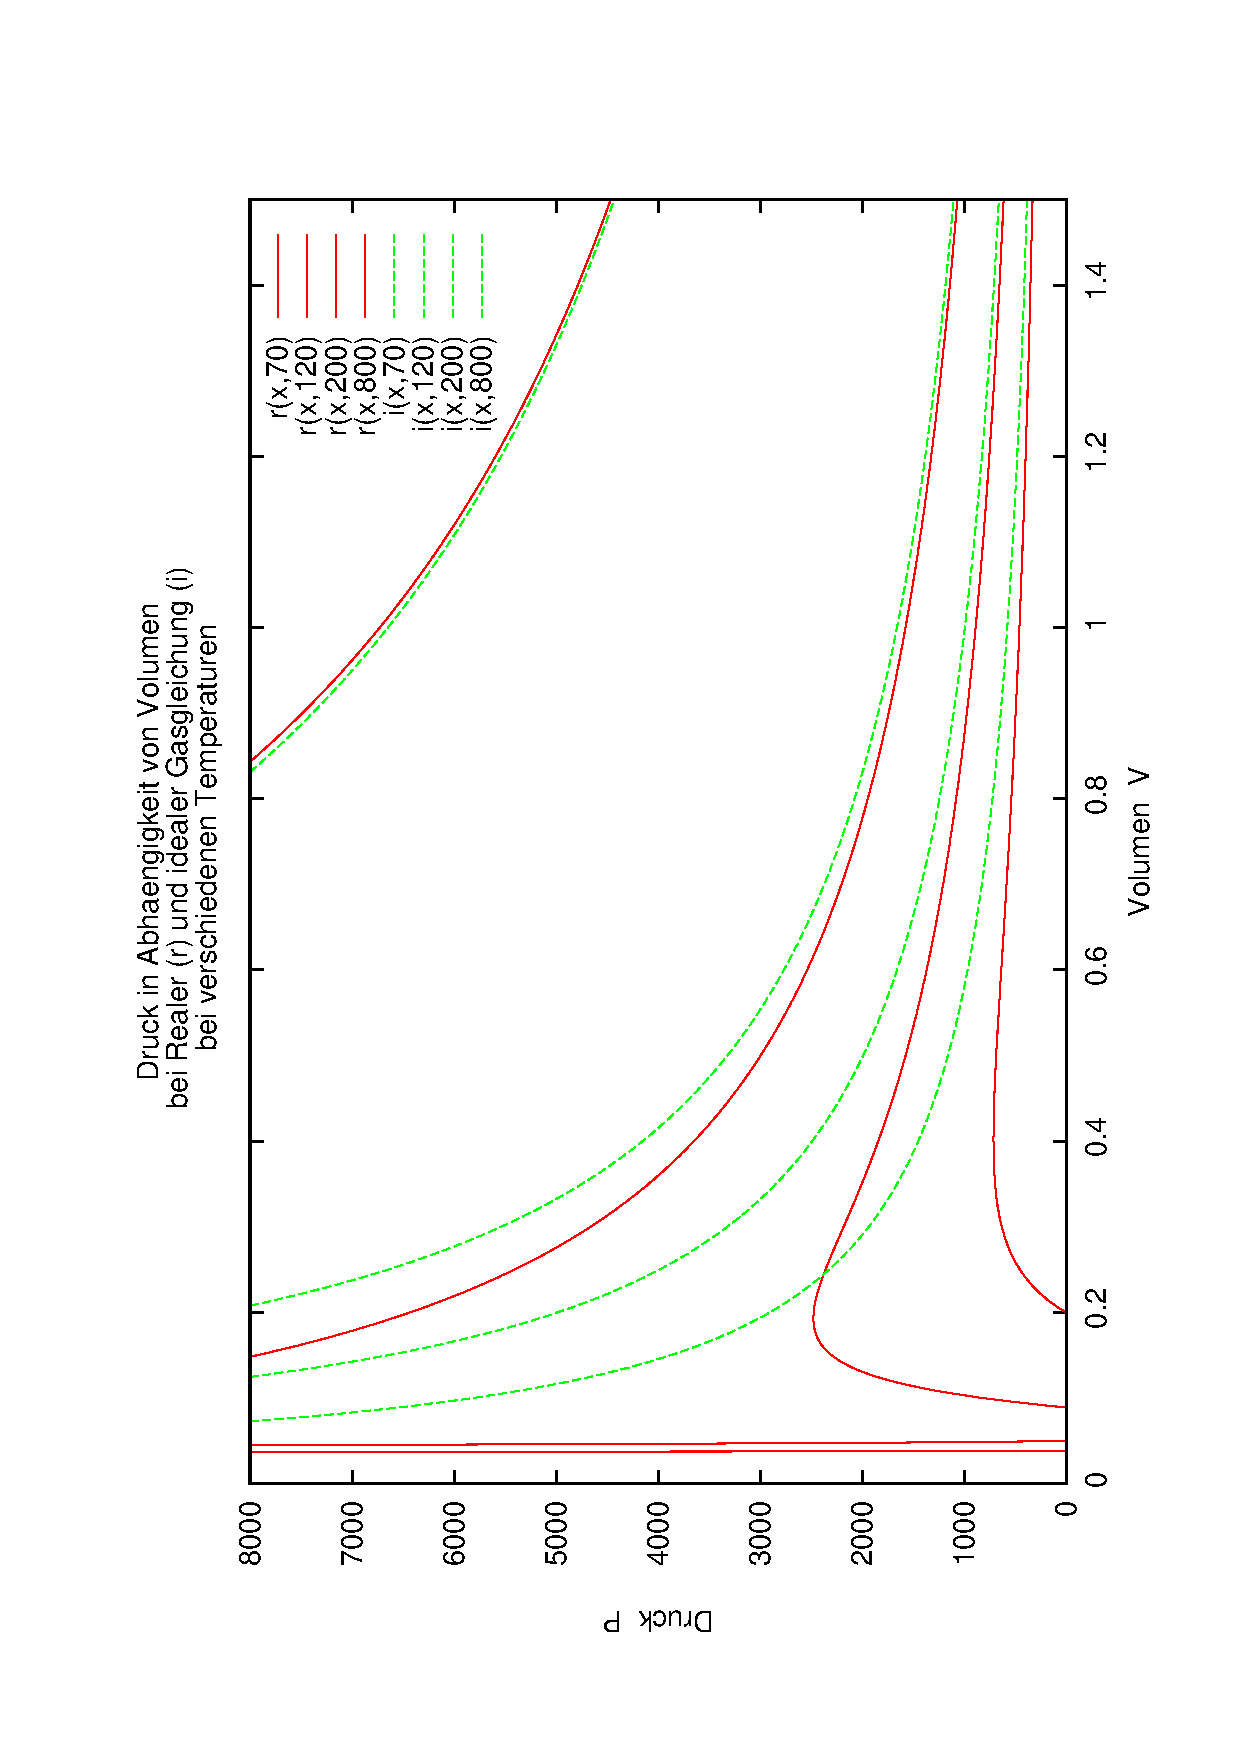
\includegraphics[width=0.7\textwidth,angle=-90]{bilder/real-ideal}}
   \subfigure[\label{abb_real_intressant}In einem interessanten
   Temperaturbereich kann man bei dem Kuververlauf des Realen Gases
   diverse Wendepunkte
   sehen]{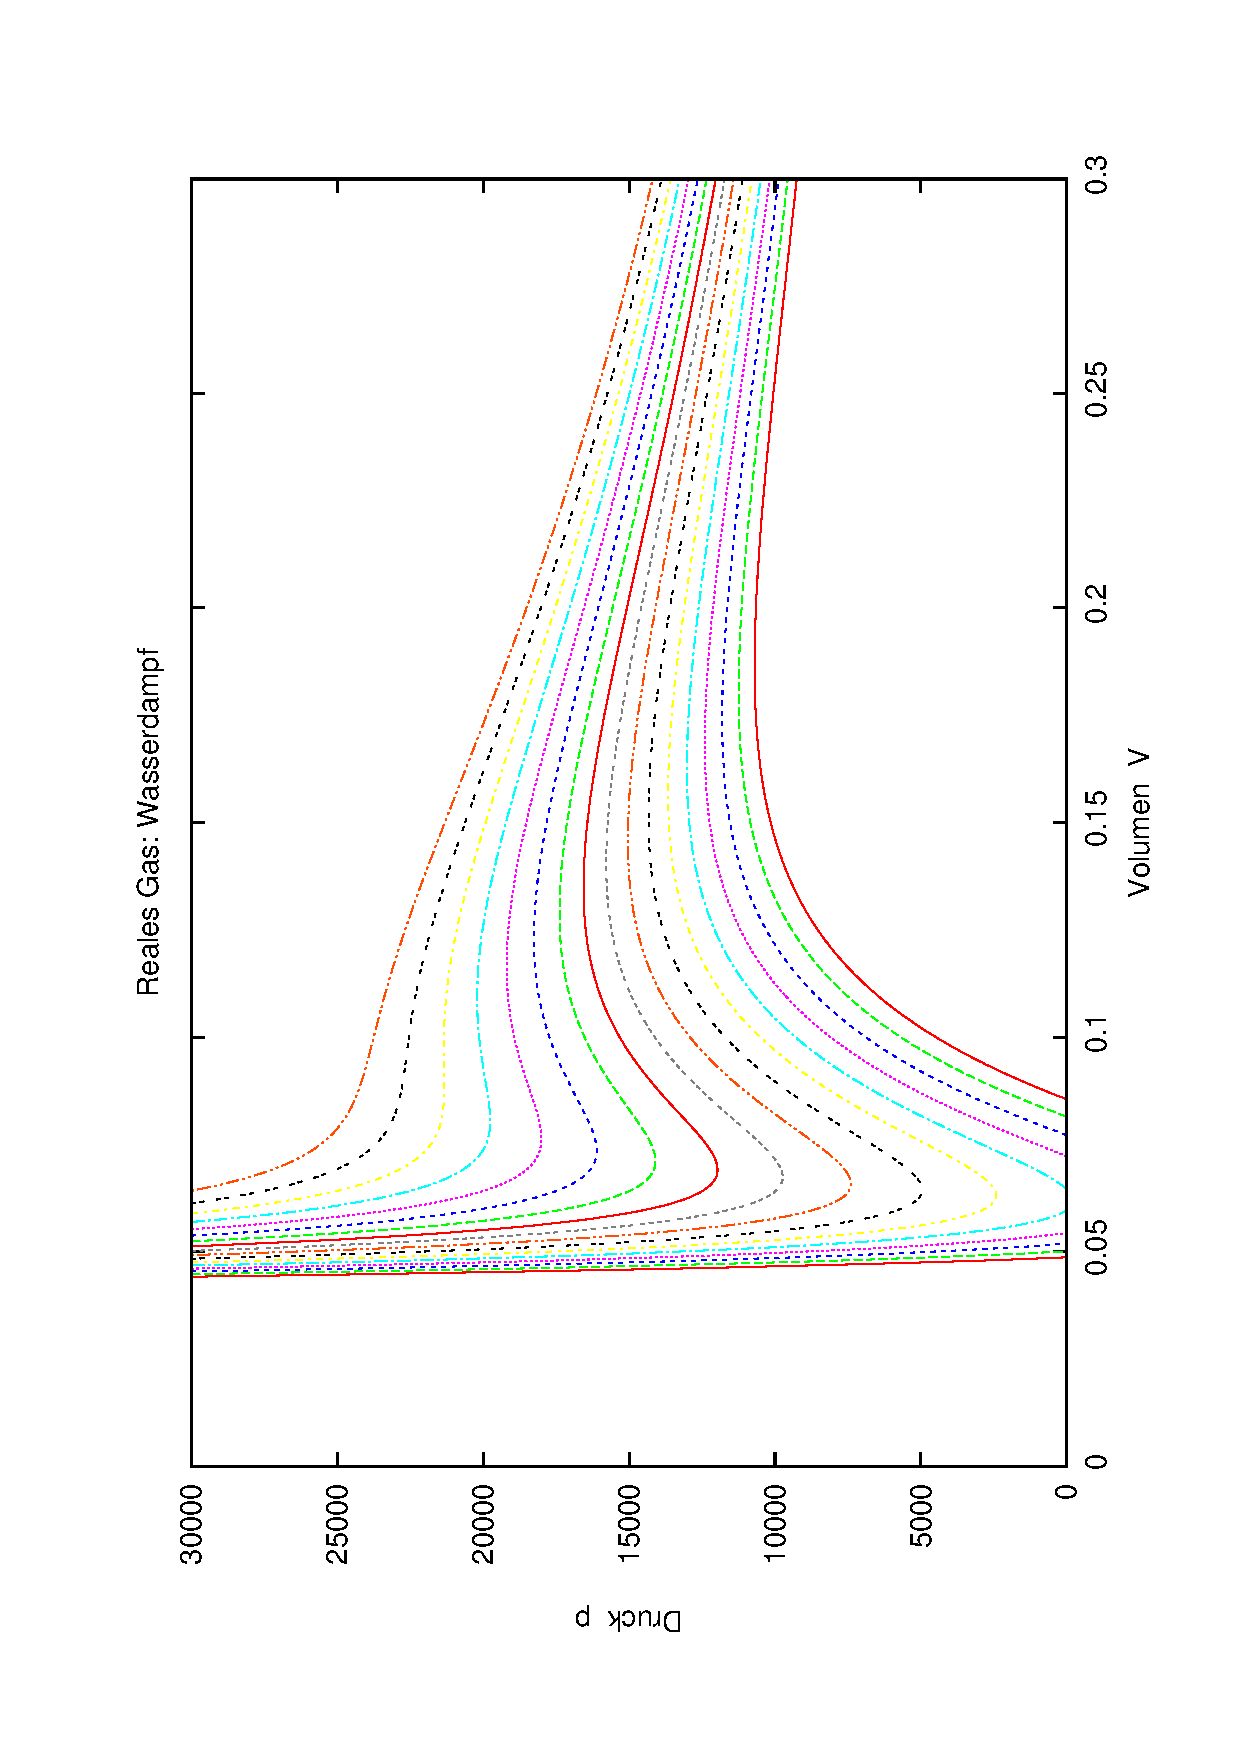
\includegraphics[width=0.7\textwidth,angle=-90]{bilder/real2}}
   \caption{Diagramme Idealer und Realer Gase}
   \label{abb_ideal-real_gas}
\end{figure}


\begin{Wichtig}
Der in Abb. \ref{abb_real_intressant} skizzierte
Verlauf tritt nur rechnerisch ein; in der Realit"at wird das nicht so
kommen:   
\end{Wichtig}
Die Wendepunkte verschwinden in der Praxis und stattdessen
werden die konkaven Abschnitte durch eine $x$-Achsen-Parallele
ersetzt, sodass die zwischen Gerade und Funktion eingeschlossenen
\emph{Orientierten Fl"achen}\footnote{also eine positive, wenn die
  Funktion gr"o"ser als die Gerade ist und eine negative, wenn die
  Funktion kleiner ist} in der Summe $0$ ergeben.
In Abb. \ref{abb_real-richtig} ist so etwas skizziert.

Die Temperatur, bei der sich gerade nur ein Wendepunkt bildet, wird
mit $T_k$ bezeichnet.\footnote{Entsprechend das entsprechende Volumen
  als $V_k$ und der dazugeh"orige Druck als $p_k$.} Wie in
Abb. \ref{abb_real-richtig} zu sehen ist, bildet sich eine Kurve, wenn
man die Punkte miteinander verbindet, die den Unterschied zwischen
Formel und Experiment markieren. Zusammen mit der Kurve mit nur einem
Wendepunkt (die also bei $T_k$ aufgenommen wurde) teilt sie das
Diagramm in Vier Abschnitte -- I bis IV -- auf:

\begin{description}[\setlabelstyle{\bfseries\slshape}]
\item[Bereich III] Das Volumen ist gro"s, der Druck jedoch klein; Das
   System bleibt \textbf{gasf"ormig}.
\item[Bereich II] Der Druck ist im Experiment konstant (deshalb die
   Konstruktion der Parallelen Linien), obwohl $V$ gr"o"ser oder kleiner
   wird.

   Die Gasteilchen kommen sich n"aher und n"aher und attraktive Kr"afte
   wirken zwischen ihnen. Manche der Gasteilchen kondensieren so und
   senken so den Druck weiter (weil die fl"ussigen Teilchen weniger
   Platz brauchen). Je weiter das Volumen reduziert wird, desto mehr
   Teilchen kondensieren, also desto mehr Fl"ussigkeit entsteht.

   Insgesamt liegt eine \textbf{Koexistenz} zwischen gasf"ormigem und
   fl"ussigem Zustand vor, die sich weiter in Richtung Fl"ussigkeit
   verschiebt, je kleiner das Volumen wird.

\item[Bereich I] Alles (oder zumindest viel Gas) ist kondensiert --
   schon f"ur geringe Volumen"anderungen ist ein sehr gro"ser Druck n"otig
   (Im Schaubild strebt die Druck-Kurve hier gegen $\infty$). Die
   Teilchen liegen also gr"o"stenteils als \textbf{Fl"ussigkeit} vor.


\item[Bereich IV] Hier befinden wir uns oberhalb der Temperatur $T_k$
   -- hier ist keine Kondensation m"oglich; die kinetisch Energie der
   Teilchen ist zu gro"s, als dass die zwischenmolekularen Kr"afte so
   stark wirken k"onnten, dass sich eine Fl"ussigkeit bildet.

Diesen Zustand nennt man \textbf{Fluid}.
\end{description}

\begin{Def} 
   [\label{def_fluid}\index{Fluid}Fluid] Ein Fluid ist eine
   Substanz, die man verformen kann, ohne dass sie einen Widerstand
   entgegen setzt. In diesem Sinne geh"oren zu den Fluiden sowohl Gase
   als auch Fl"ussigkeiten.
\end{Def}

Diese Verallgemeinerung macht Sinn, weil viele physikalische Gesetze
f"ur Gase und Fl"ussigkeiten (qualitativ) gleicherma"sen gelten und
die Eigenschaften sich nur quantitativ unterscheiden.

Mit anderen Worten: Es macht hier keinen Sinn, zwischen Fl"ussigkeit
und Gas zu unterscheiden, deshalb nenne man den Zustand Fluid.

In Tabelle \ref{tab_Tk} sind ein paar der kritischen Temperaturen
aufgef"uhrt, wie sie im Experiment vorkommen.

\bigskip
\noindent

So kann man auch noch ein
sog. \textbf{\index{Phasendiagramm}Phasendiagramm} zeichnen. In ihm
wird genau festgehalten, wie das \emph{Verh"altnis von Druck und
  Temperatur} sein muss, damit man eine bestimmte Phase erh"alt. In
Abb. \ref{abb_pasendiagramm} ist ein solches
dargestellt.\footnote{Bitte beachten: dies ist ein $p$-$T$-Diagramm;
  man kann es nur schwer mit den $p$-$V$-Diagrammen wie
  \ref{abb_ideal-real_vgl} oder \ref{abb_real-richtig} vergleichen!} 

Um die Kurve, welche den fl"ussigen vom gasf"ormigen Zustand eines Mols Gas
trennt (auch \emph{Siedekurve} genannt) zu berechnen, verwendet man
$$
p(T) = p_0 \cdot \exp \frac{-Q_D}{RT}
$$
wobei mit $Q_D$ die \emph{Verdampfungsw"arme} eines Mols der Teilchen ist.






\begin{figure}[h]
   \centering
   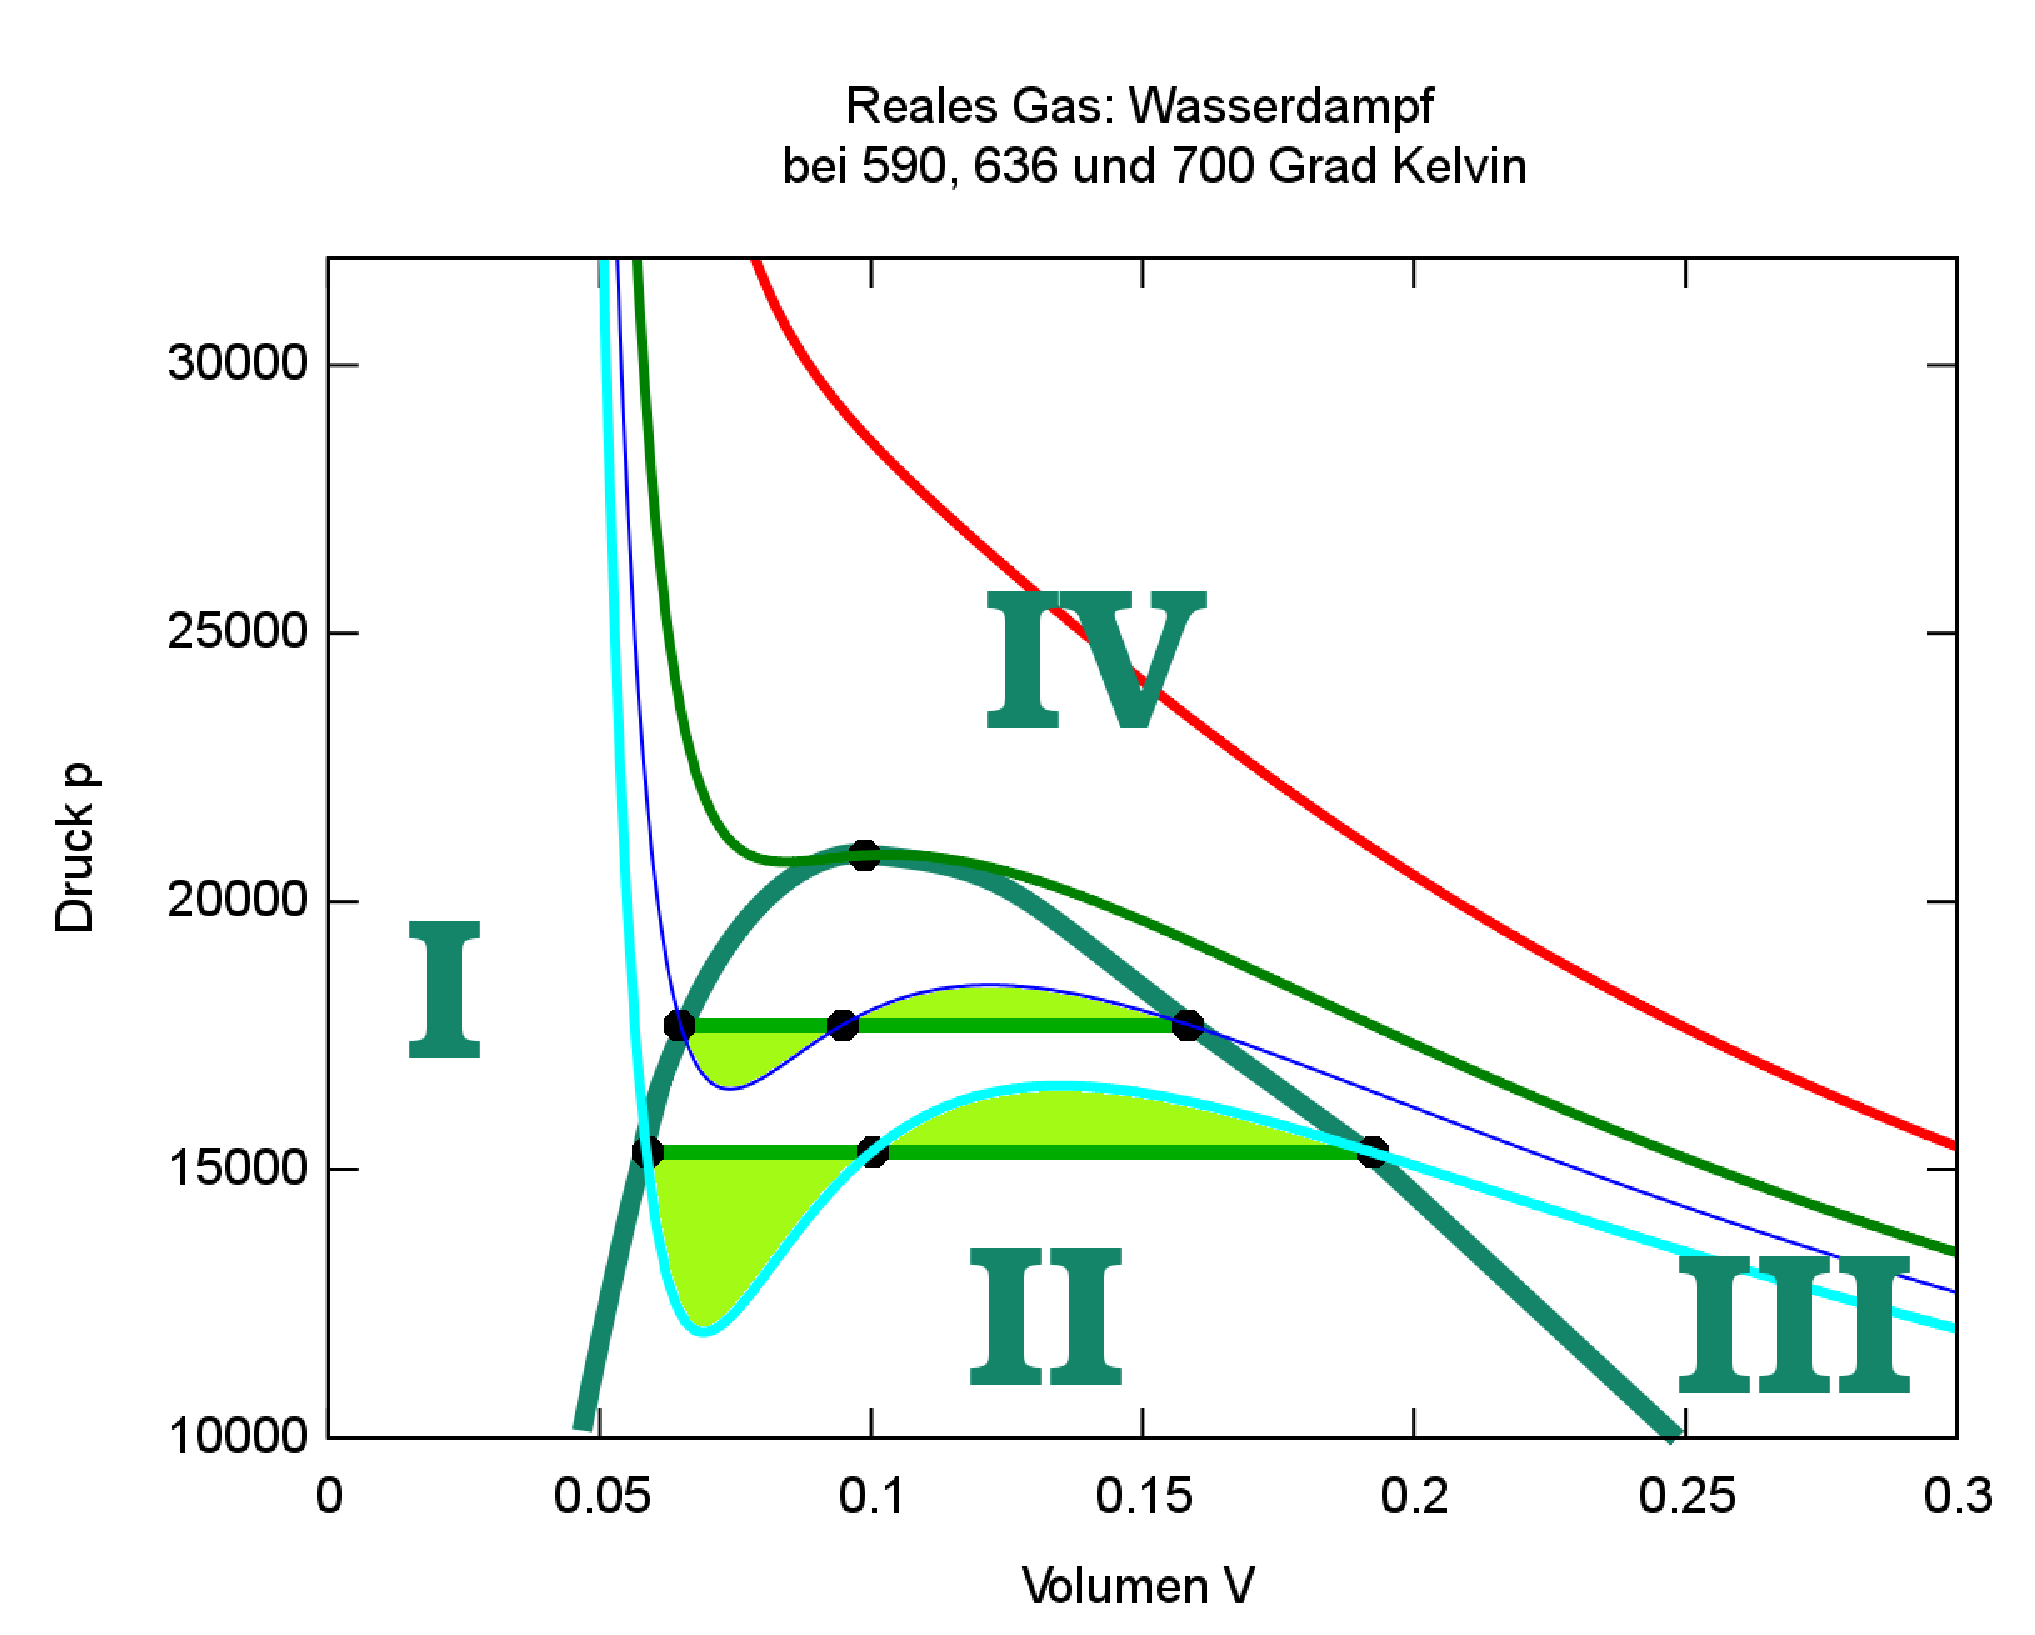
\includegraphics[width=12cm]{bilder/real2c_mod2}
   \caption[p-V-Diagramm reales Gas]{Realer Kurvenverlauf skizziert,
     mit diversen Konstruktionshilfen und den gebieten I bis IV
     eingezeichnet.}
   \label{abb_real-richtig}
\end{figure}



\begin{table}[h]
   \centering
   \begin{tabular}{l | r r r}
\toprule
      ~ & $\mathbf{p_k}$ in bar & $\mathbf{T_k}$ in K &
      $\mathbf{\varrho_k}$ in
      $\frac{\operatorname{kg}}{\operatorname{m}^3}$ \\
\midrule
      $H_2$ & 12,9 & 33,2 & 31\\
      $CO_2$ & 73,7 & 304,1 & 465 \\
      $H_2O$ & 221,0 & 647,3 & 317 \\
\bottomrule
   \end{tabular}
   \caption{Tabelle kritischer Dampfdr"ucke, Temperaturen und Dichten von Gasen}
   \label{tab_Tk}
\end{table}


\begin{figure}
   \centering
   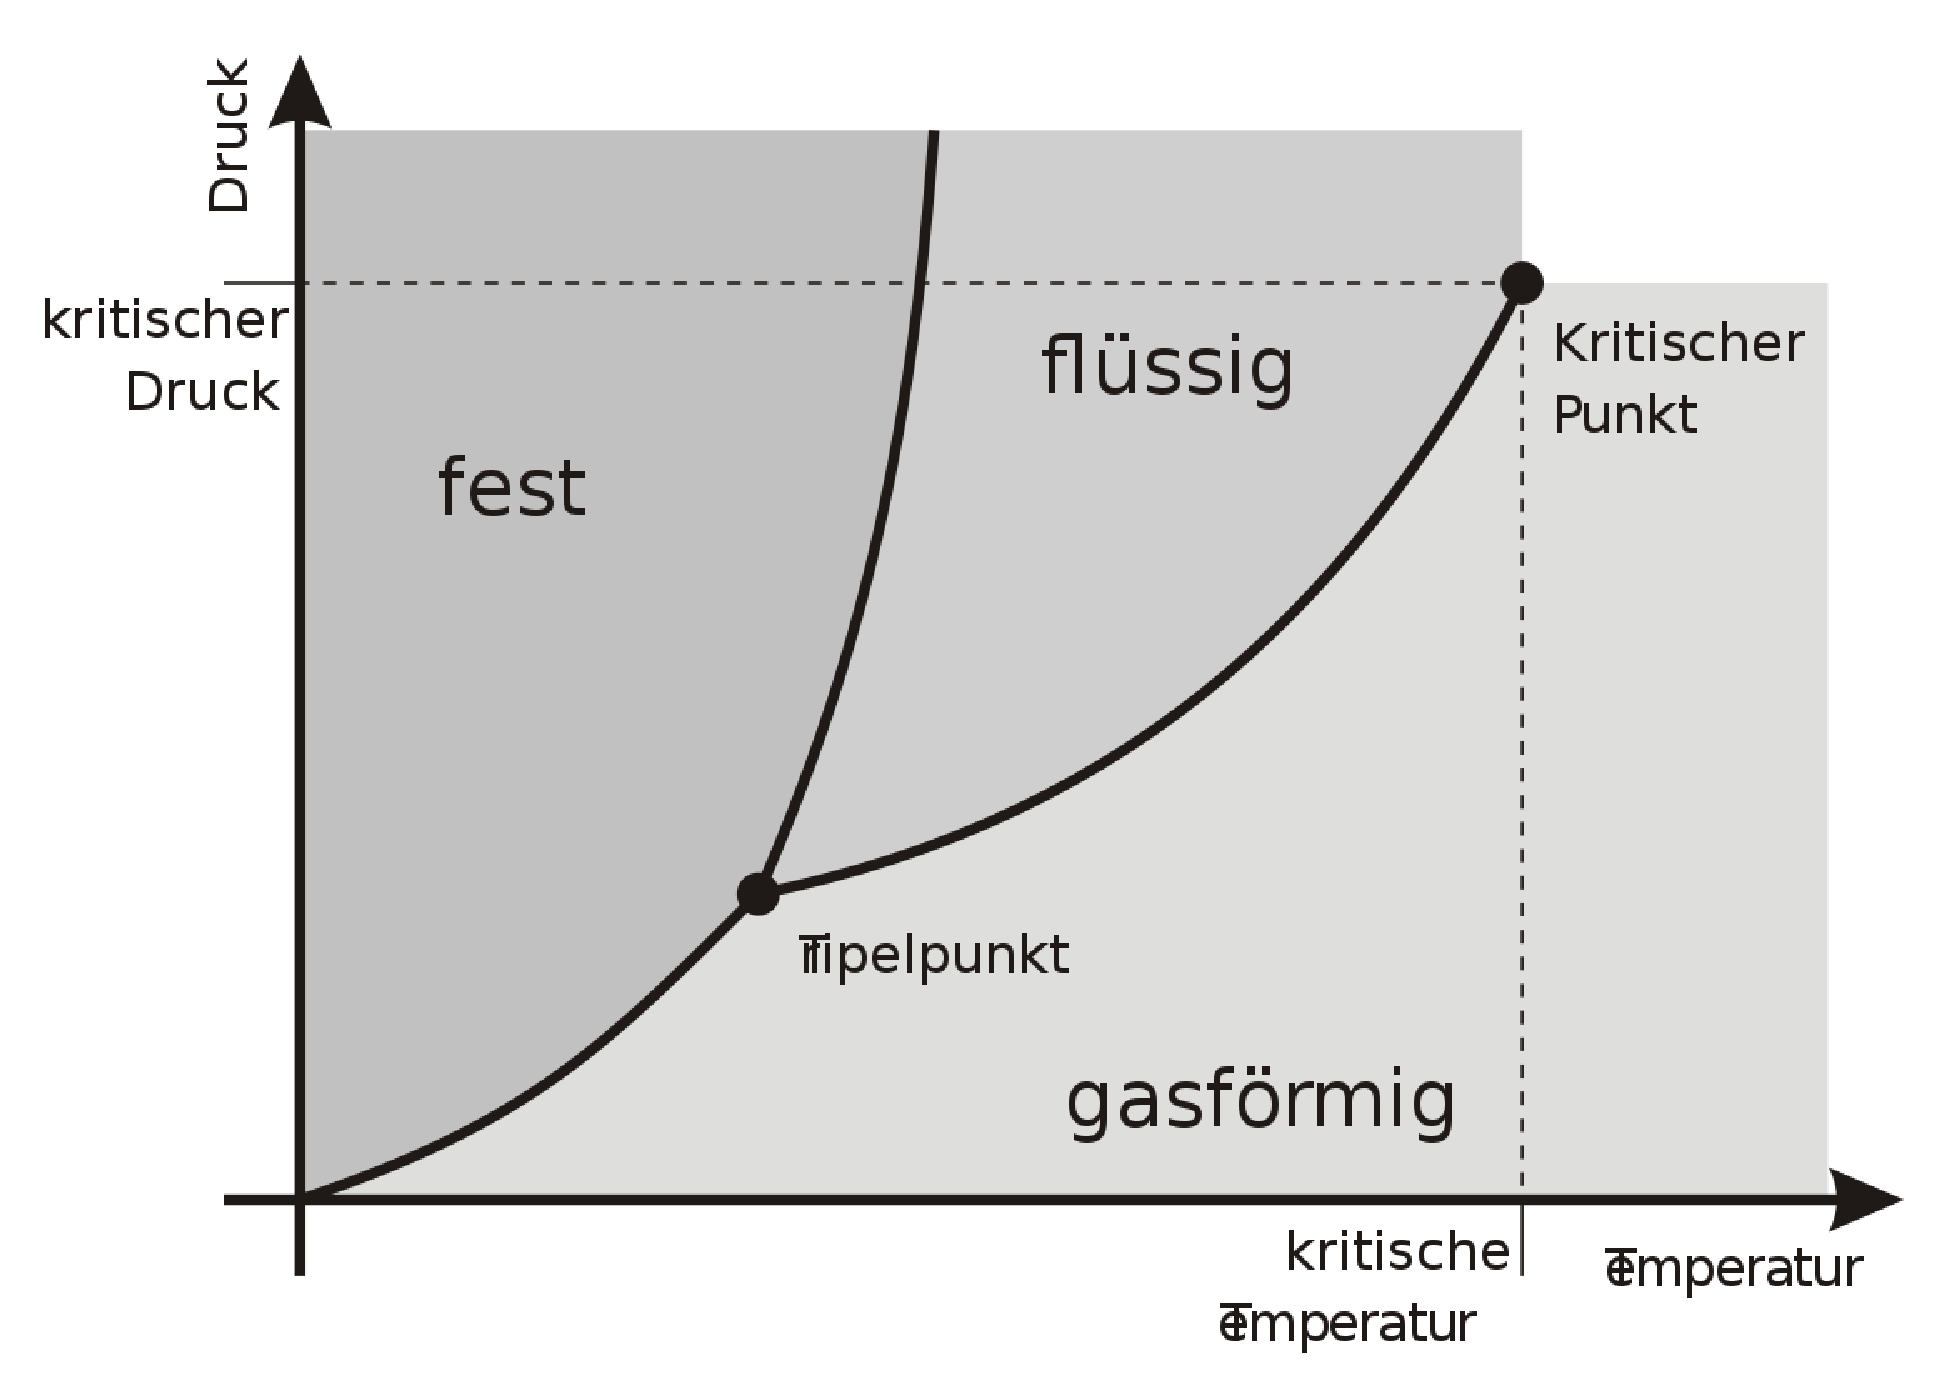
\includegraphics[width=0.6\textwidth]{bilder/phasen}
   \caption[Phasendiagramm: reales Gas]{Phasendiagramm eines realen Stoffes (ohne Anomalie -- also nicht wie
Wasser). (Quelle: \textsc{Wikipedia})}
   \label{abb_pasendiagramm}
\end{figure}




\clearpage

\section[\textsc{Guggenheim}-Quadrat]{Das \textsc{Guggenheim}-Quadrat (und seine Vergewaltigung) $(\bigstar)$}
\label{kap_guggenheim-quadrat-und-seine-vergewaltigung}



\begin{figure}
   \centering
   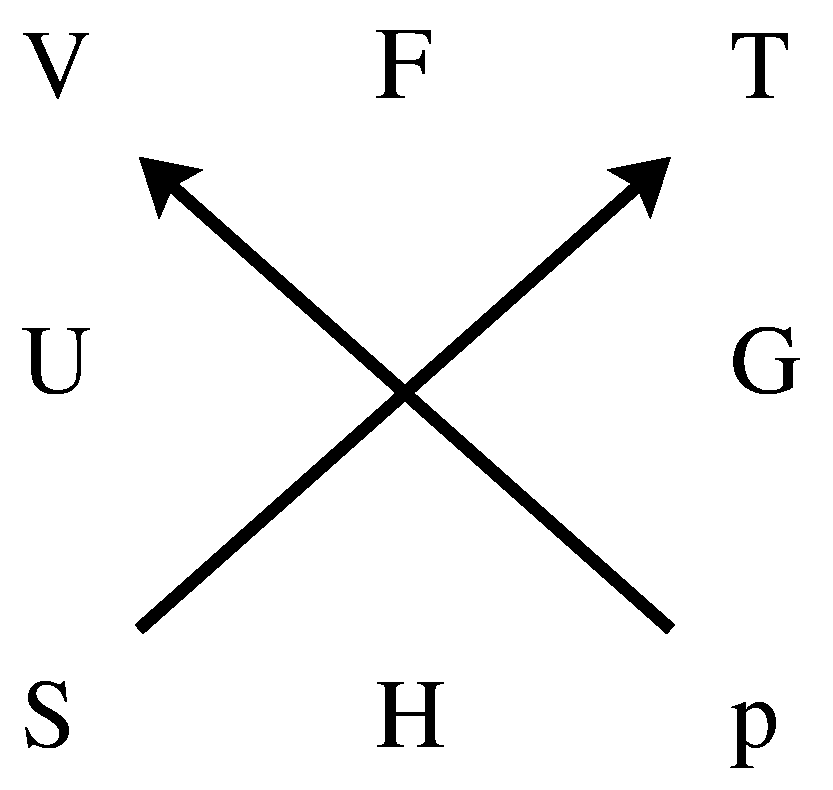
\includegraphics[width=0.6\textwidth]{bilder/guggenheim}
   \caption{Das \textsc{Guggenheim}-Schema}
   \label{abb_guggenheim}
\end{figure}


In Abb. \ref{abb_guggenheim} ist das \textsc{\index{Guggenheim
    Schema}Guggenheim}-Schema dargestellt. Es erm"oglicht, sich
zahlreiche Zusammenh"ange der Thermodynamischen Gr"o"sen (mit geringem
Aufwand) zu merken.

Darin stehen die Buchstaben f"ur: S: Entropie, V: Volumen, T:
Temperatur, p: Druck, H: Enthalpie, U: Innere Energie, F: Freie
Energie und G: Gibbs'sche Enthalpie. Um sich dieses Schema merken zu
k"onnen, gibt es einen sch"onen Merkspruch:
\begin{quote}
   \textbf{S}o \textbf{V}iel \textbf{T}hermo-\textbf{P}hysik
   \textbf{H}"atte \textbf{U}ns \textbf{F}ast \textbf{G}eschafft!
\end{quote}
Dabei f"angt man in der linken unteren Ecke an und schreibt im
Uhrzeigersinn die vier Zustandstr"o"sen S, V, T und p an und beginnt
direkt hinter p mit den restlichen Gr"o"sen. Die Pfeile haben
anschlie"send eine wichtige Bedeutung.

Es gelten nun folgende "`Gebrauchsanweisungen"':
\begin{description}[\setlabelstyle{\bfseries\slshape}]
\item[Ableitungen] Um Partielle Ableitungen der Gr"o"sen nacheinander zu
   gewinnen, gilt die Formel:
   \begin{equation}
      \label{eq:430}
      \left ( \frac{\partial <\text{Kante}>}{\partial <\text{Ecke}>} \right )_{<\text{Ecke
          des Dreiecks}>} = \pm <\text{Pfeil folgen}>
   \end{equation}
D.h. man W"ahlt eine Gr"o"se auf der Kante $X$ (bspw. $H$) und bewegt sich zu
einem anliegenden Eck $Y$ (bspw. $S$) um die partielle Ableitung
$\frac{\partial X}{\partial Y}$ zu bestimmen. Nun folgt man dem Pfeil
zur n"achsten Ecke und erh"alt hier die Gr"o"se $Z$ rechts der
Gleichung. Wenn man dabei \emph{mit} dem Pfeil gegangen ist, ist das
Vorzeichen \emph{positiv}, \emph{entgegen} dem Pfeil, ist es
\emph{negativ}. Bei der Ableitung hat eine Gr"o"se konstant zu bleiben:
Dabei handelt es sich um die Ecke $W$, welche zusammen mit den bisher
gew"ahlten Gr"o"sen ein rechtwinklig, gleichschenkliges Dreieck
bildet. Es ist dann:
\begin{equation*}
\left (   \frac{\partial X}{\partial Y} \right )_W = \pm Z
\end{equation*}
Und so bspw:
\begin{equation*}
   \left ( \frac{\partial H}{\partial S} \right )_p = T 
\text{ oder }
\left ( \frac{\partial H}{\partial p} \right )_S = V
\text{ oder }
\left ( \frac{\partial U}{\partial V} \right )_S = -p
\end{equation*}
F"ur diese Aufgabe ist das Schema eigentlich gemacht, deshalb stimmen
hier die Pfeilrichtungen mit $+$ und $-$ "uberein.
\item[Totale Differenziale] 
So kann man die totalen Differenziale einer der \textbf{Kanten}
bestimmen:
\begin{equation}
   \label{eq:431}
 \diff  <\text{K.}> = \pm <\text{E. gegen"uber}> \diff
 <\text{P. folg.}> \pm <\text{andere E.}> \diff <\text{P. folg.}>
\end{equation}
D.h. man w"ahlt eine Kante und geht von dieser zur gegen"uberliegenden
Ecke und mulipliziert diese Gr"o"se mit dem Differenzial der Gr"o"se, zu
der man gelangt, wenn man dem Pfeil folgt (in der endg"ultigen Formel
sind also die Gr"o"sen aller drei Differenziale Nachbarn im
\textsc{Guggenheim}-Quadrat). Das Vorzeichen ist dabei ist \emph{mit}
der Pfeilrichtung \emph{negativ} und \emph{entgegen} der Pfeilrichtung
positiv. Wichtig ist dabei, dass man \emph{beide} gegen"uberliegende
Ecken enbezieht, also im Endeffekt alle vier Zustandsgr"o"sen gebraucht
hat.

Bspw. gilt:
\begin{equation*}
   \diff H = T \diff S + V \diff p \text{ oder } \diff G = V \diff p -
   S \diff T
\end{equation*}
\item[\textsc{Maxwell}-Beziehungen] 
Hier kann man die Ecken gegeneinander partiell ableiten. Es gilt:
\begin{equation}
   \label{eq:432}
   \left ( \frac{\partial <\text{E.1}>}{\partial <\text{E.2}>} \right
   )_{<\text{Nenner gegen"ub.}>} = \left ( \frac{\partial
        <\text{P. folgen}>}{\partial <\text{letze E.}>} \right
   )_{<\text{Nenner gegen"ub.}>}
\end{equation}
Dabei w"ahlt man die ersten beiden Ecken frei aus und bildet die linke
Ableitung.  Dann folgt
man dem Pfeil (von $<\text{E.2}>$) zur n"achsten Ecke und bildet mit
dieser und der letzten Ecke die rechte Ableitung. Dabei ist bei der
linken Ableitung die Gr"o"se Konstant, die Rechts im Nenner steht und
anderst herum.  Auf einer der Seiten \emph{sowohl} $S$ als auch $p$
auftauchen (diese liegen beide an den stumpfen Pfeilenden), dann kommt
vor diese Ableitung ein "`$-$"', sonst \emph{nicht}.

Also bspw.:
\begin{equation*}
   \left ( \frac{\partial V}{\partial T} \right )_p = - \left (
      \frac{\partial S}{\partial p} \right )_T
\text{ oder }
\left ( \frac{\partial T}{\partial p} \right )_S = \left ( \frac{\partial V}{\partial S} \right )_p
\end{equation*}

\item[Definitionen] 
Man kann die drei Definitionen 
\begin{eqnarray*}
   \mathcal F &=& U - TS ~  \text{ eigentlich } U = \mathcal F + TS\\
G &=& H - TS \\
H &=& U + pV
\end{eqnarray*}
(mit ein wenig Gewalt) in das Schema pressen:
\begin{equation}
   \label{eq:433}
<\text{K.}> = <\text{n"achste K.}> \pm <\text{n"achste E.}> \cdot
<\text{P. folgen}>
\end{equation}
% Man w"ahlt also eine Kante und bewegt sich zur n"achsten Kante. Die
% "`n"achste"' ist im Falle von $G$ und $H$ im Uhrzeigensinn und bei
% $\mathcal F$ im \emph{Gegen}uhrzeigersinn.
Man w"ahlt also eine Kante und bewegt sich zur n"achsten Kante im
Uhrzeigersinn, weiter zur n"achsten Ecke und folgt hier dem Pfeil.
Das Vorzeichen ist wieder positive, wenn man \emph{gegen} den Pfeil
geht und \emph{mit} dem Pfeil \emph{negativ}.
\end{description}

\abs
Man kann diese Relationen herleiten, indem man bekannte Gr"o"sen per
\textbf{Legendre}-Transformation transformiert (damit kann man elegant
die totalen Differenziale umschreiben) und erh"alt durch
Koeffizientenvergleiche die Ableitungen $\frac{\partial
  <\text{Kante}>}{\partial <\text{Ecke}>}$.

Mit diesen Grundgleichungen zusammen mit $\bar u = \frac{f}{2} K_B T$
kann man viele der hier besprochenen F"alle schnell und einfach nachrechnen!





















